% =============================================================================
% Poliscope 技术白皮书（第二版）
% 编译：xelatex tech.tex（连续两遍以生成目录与交叉引用）
% =============================================================================
\documentclass[11pt]{ctexart}

% ---------- 页面 ----------
\usepackage[a4paper, top=2.5cm, bottom=2.4cm, left=2.6cm, right=2.6cm]{geometry}
\usepackage{microtype}
\usepackage[table]{xcolor}
\usepackage{fontspec}
\usepackage{amsmath}
\usepackage{amssymb}
\usepackage{booktabs}
\usepackage{tabularx}
\usepackage{array}
\usepackage{enumitem}
\usepackage{needspace}
\usepackage{caption}
\usepackage[most]{tcolorbox}
\usepackage{tikz}
\usetikzlibrary{positioning, arrows.meta, shapes.geometric, fit, backgrounds, calc}
\usepackage{titlesec}
\usepackage{tocloft}
\usepackage{fancyhdr}
\usepackage[colorlinks=true, linkcolor=accent, urlcolor=accent, citecolor=accent]{hyperref}

% ---------- 设计令牌：配色 ----------
\definecolor{ink}{HTML}{17202B}        % 主文字 / 标题
\definecolor{ink2}{HTML}{3C4756}       % 次级文字
\definecolor{muted}{HTML}{6A7482}      % 弱化文字
\definecolor{accent}{HTML}{1F5C99}     % 唯一主强调色（钢蓝）
\definecolor{accentdk}{HTML}{174674}   % 强调色加深
\definecolor{tint}{HTML}{EBF2F9}       % 强调色浅底
\definecolor{panel}{HTML}{F5F7FA}      % 面板浅底
\definecolor{linegray}{HTML}{D7DEE7}   % 发丝线
\definecolor{okgreen}{HTML}{2E7D5B}
\definecolor{tintgreen}{HTML}{EAF4EF}
\definecolor{warnamber}{HTML}{9A6B16}
\definecolor{tintamber}{HTML}{FAF4E6}
\definecolor{riskred}{HTML}{A63D3A}
\definecolor{coverbg}{HTML}{11151B}    % 封面近黑
\definecolor{coverrule}{HTML}{3A4656}

% ---------- 字体 ----------
\setmainfont{TeX Gyre Heros}[Scale=0.96]
\setmonofont{TeX Gyre Cursor}[Scale=0.92]
\setCJKmainfont{Microsoft YaHei}[BoldFont={Microsoft YaHei Bold}]
\setCJKsansfont{Microsoft YaHei}[BoldFont={Microsoft YaHei Bold}]
\linespread{1.22}\selectfont
\color{ink}
\setlength{\emergencystretch}{3em}\tolerance=1400\hbadness=2000

% ---------- 标题样式 ----------
\titleformat{\section}
  {\sffamily\bfseries\fontsize{17}{22}\selectfont\color{ink}}
  {\colorbox{accent}{\color{white}\enspace\thesection\enspace}}{0.7em}
  {}
  [\vspace{2pt}{\color{linegray}\titlerule[1pt]}]
\titlespacing*{\section}{0pt}{1.5em}{0.9em}

\titleformat{\subsection}
  {\sffamily\bfseries\fontsize{12.5}{16}\selectfont\color{ink}}
  {\textcolor{accent}{\rule[0.12em]{0.52em}{0.52em}}}{0.6em}
  {}
\titlespacing*{\subsection}{0pt}{1.2em}{0.45em}

\titleformat{\subsubsection}
  {\sffamily\bfseries\fontsize{11}{14}\selectfont\color{ink2}}
  {}{0em}{}
\titlespacing*{\subsubsection}{0pt}{0.9em}{0.3em}

\setcounter{tocdepth}{2}

% ---------- 目录 ----------
\renewcommand{\cftsecfont}{\sffamily\bfseries\color{ink}}
\renewcommand{\cftsecpagefont}{\sffamily\bfseries\color{ink}}
\renewcommand{\cftsubsecfont}{\sffamily\color{ink2}}
\renewcommand{\cftsubsecpagefont}{\sffamily\color{ink2}}
\renewcommand{\cftsecdotsep}{\cftdotsep}
\renewcommand{\cftsecleader}{\sffamily\color{muted}\cftdotfill{\cftdotsep}}
\renewcommand{\cftsubsecleader}{\sffamily\color{muted}\cftdotfill{\cftdotsep}}
\setlength{\cftbeforesecskip}{5pt}

% ---------- 页眉页脚 ----------
\pagestyle{fancy}
\fancyhf{}
\fancyhead[L]{\sffamily\footnotesize\color{muted}Poliscope 技术白皮书}
\fancyhead[R]{\sffamily\footnotesize\color{muted}\thepage}
\renewcommand{\headrulewidth}{0.6pt}
\renewcommand{\headrule}{\hbox to\headwidth{\color{linegray}\leaders\hrule height \headrulewidth\hfill}}
\setlength{\headheight}{14pt}

% ---------- 内容盒子 ----------
\newtcolorbox{principlebox}[1][]{
  colback=tint, colframe=accent, boxrule=0pt, leftrule=3pt,
  arc=1.5pt, outer arc=1.5pt, left=10pt, right=10pt, top=8pt, bottom=8pt,
  fonttitle=\sffamily\bfseries, coltitle=white,
  breakable, #1}
\newtcolorbox{mechbox}[1][]{
  colback=panel, colframe=linegray, boxrule=0pt, leftrule=3pt,
  arc=1.2pt, outer arc=1.2pt, left=10pt, right=10pt, top=7pt, bottom=7pt,
  breakable, #1}
\newtcolorbox{honestbox}[1][]{
  colback=tintamber, colframe=warnamber, boxrule=0pt, leftrule=3pt,
  arc=1.2pt, outer arc=1.2pt, left=10pt, right=10pt, top=7pt, bottom=7pt,
  breakable, #1}
\newtcolorbox{findingbox}[1][]{
  colback=tintgreen, colframe=okgreen, boxrule=0pt, leftrule=3pt,
  arc=1.2pt, outer arc=1.2pt, left=10pt, right=10pt, top=7pt, bottom=7pt,
  breakable, #1}

% 统一的小标签
\newcommand{\boxtag}[1]{{\sffamily\bfseries\footnotesize #1}\par\vspace{2pt}}

% ---------- 表格 ----------
\captionsetup{font={small,sf}, labelfont={bf,sf}, labelsep=quad}
\newcommand{\thd}[1]{{\sffamily\bfseries #1}}
\newcolumntype{L}[1]{>{\raggedright\arraybackslash}p{#1}}
\renewcommand{\arraystretch}{1.32}
\newcommand{\tblhead}{\color{white}\sffamily\bfseries}

% ---------- 代码 ----------
\usepackage{listings}
\lstset{
  basicstyle=\ttfamily\footnotesize\color{ink},
  keywordstyle=\sffamily\bfseries\color{accentdk},
  commentstyle=\itshape\color{muted},
  stringstyle=\color{accentdk},
  numberstyle=\tiny\color{muted},
  breaklines=true,
  frame=none,
  backgroundcolor=\color{panel},
  columns=flexible,
  xleftmargin=8pt, xrightmargin=8pt,
  aboveskip=0.7em, belowskip=0.7em,
  showstringspaces=false,
  tabsize=2,
}
\lstdefinelanguage{ps}{morekeywords={def,return,if,else,elif,for,in,not,and,or,None,True,False,class,import,from,try,except,raise,with,as,while,lambda}}

% ---------- TikZ 共享样式 ----------
\tikzset{
  nd/.style={rounded corners=2.5pt, draw=linegray, line width=0.7pt,
    fill=white, text=ink, font=\sffamily\scriptsize, align=center,
    inner sep=4.5pt, minimum height=2.2em},
  nda/.style={nd, draw=accent, fill=tint, text=accentdk, font=\sffamily\bfseries\scriptsize},
  ndd/.style={nd, fill=ink, text=white, draw=ink, font=\sffamily\bfseries\scriptsize},
  flow/.style={-{Stealth[length=2.2mm]}, line width=0.8pt, color=accent},
  flowg/.style={-{Stealth[length=2.2mm]}, line width=0.7pt, color=muted, dashed},
  lbl/.style={font=\sffamily\tiny\color{muted}, align=center},
}

% ---------- 通用小命令 ----------
\newcommand{\code}[1]{{\ttfamily\footnotesize #1}}
\newcommand{\seat}[1]{{\ttfamily\footnotesize #1}}

\begin{document}

% ============================== 封面 ==============================
\begin{titlepage}
\thispagestyle{empty}
\begin{tikzpicture}[remember picture, overlay]
  \fill[coverbg] (current page.south west) rectangle (current page.north east);
  % 顶部标识带
  \draw[coverrule, line width=0.8pt] ([xshift=2.6cm,yshift=-2.6cm]current page.north west)
    -- ([xshift=-2.6cm,yshift=-2.6cm]current page.north east);
  \node[anchor=west, text=white, font=\sffamily\bfseries\footnotesize]
    at ([xshift=2.6cm,yshift=-2.28cm]current page.north west) {POLISCOPE\enspace\textcolor{muted}{\textbar}\enspace\textcolor{muted}{研究智能体技术文件}};
  % 底部信息带
  \draw[coverrule, line width=0.8pt] ([xshift=2.6cm,yshift=3.05cm]current page.south west)
    -- ([xshift=-2.6cm,yshift=2.9cm]current page.south east);
\end{tikzpicture}

\vspace*{3.2cm}
{\sffamily\color{white}\fontsize{46}{50}\selectfont\bfseries Poliscope\par}
\vspace{0.55cm}
{\sffamily\color{white!85}\fontsize{20}{26}\selectfont 技术白皮书\par}
\vspace{0.35cm}
\textcolor{accent}{\rule{4.2cm}{2.4pt}}\par
\vspace{1.1cm}
{\sffamily\color{white!92}\fontsize{15.5}{24}\selectfont\bfseries
EpistemoBrain：七人科学议会、双图证据治理\\与计算社会科学盲点发现智能体\par}
\vspace{0.9cm}
{\sffamily\color{white!60}\fontsize{10.5}{16}\selectfont
七名 AI 科学家独立取证、交叉质询、专门寻找反例，\\
产出结论与局限并排、证据可溯源、异议不删除的争议证据地图。\par}

\vfill
\begin{tikzpicture}[remember picture, overlay]
  \node[anchor=south west, text=white!55, font=\sffamily\footnotesize]
    at ([xshift=2.6cm,yshift=2.45cm]current page.south west)
    {版本 2.0\quad\textbar\quad2026 年 9 月\quad\textbar\quad MIT License};
  \node[anchor=south west, text=white!55, font=\sffamily\footnotesize]
    at ([xshift=2.6cm,yshift=1.78cm]current page.south west)
    {源码仓库：github.com/Fishman-free/poliscope\quad\textbar\quad 在线实例：poliscope.tech};
  \node[anchor=south west, text=white!55, font=\sffamily\footnotesize]
    at ([xshift=2.6cm,yshift=1.11cm]current page.south west)
    {配套学术论文：EpistemoBrain（ACL Findings 2026 格式，源码见 docs/paper/）};
\end{tikzpicture}
\end{titlepage}

% ============================== 摘要 ==============================
% ===================== 执行摘要 =====================
\thispagestyle{fancy}
{\sffamily\bfseries\fontsize{20}{24}\selectfont\color{ink} 执行摘要\par}
\vspace{0.5em}
\noindent{\color{linegray}\rule{\linewidth}{1pt}}
\vspace{1em}

大型语言模型让「输入问题、自动产出研究综述」变得触手可及，但在存在争议的科研问题上，标准深度研究管线有三个文风优化无法修复的缺陷：\textbf{单一视角}——管线里没有测量学家，自报告偏差就无人指出；\textbf{重复即共识的错觉}——多个智能体读到同一份错误摘要，共享的错误会被包装成「被反复验证」；\textbf{总结器拍平异议}——最后一步「大家基本同意」抹掉了争议研究最该保留的少数意见与证伪条件。

\medskip
Poliscope 面向计算社会科学争议问题（首版领域：数字行为、社交媒体与心理健康），给出的回答是 \textbf{EpistemoBrain}：一套由七名专业化 AI 科学家、三层科研记忆和双图证据治理组成的研究组织方法，以及它的完整开源实现。本文档说明这套方法的机制、工程实现、评测证据与已知边界。

\subsection*{\sffamily\color{accentdk}三条核心创新}

\begin{enumerate}[leftmargin=1.6em, itemsep=4pt, topsep=4pt]
\item \textbf{七人科学议会（Council Protocol）。}七个固定席位按八阶段协议工作，只允许提交八类结构化科研动作；协议明确禁止多数投票裁决科研真理，最终产物是保留具名异议与证伪条件的条件化共识，而不是「6:1 通过」。
\item \textbf{双图证据治理（Dual-Graph Governance）。}过程图与证据图物理分离，所有正式修改先进入追加写、幂等、可重放的科学事件账本，再由数据库层唯一有权限的图投影器写入证据图。过程材料在结构上不可能自动升级为证据。
\item \textbf{可证伪的实现与评测。}系统以模块化单体完整落地（14 个内部包、4 个应用、43 个数据库迁移、1187 项自动化测试），并配套 ForesightBlindspot 时间切片评测协议：五条能力递增基线、六项单机制消融，真实模型上的对照结果与其失败边界一并公开。
\end{enumerate}

\subsection*{\sffamily\color{accentdk}关键事实}

\vspace{0.4em}
\begin{tcolorbox}[colback=white, colframe=linegray, boxrule=0.8pt, arc=2pt, left=8pt,right=8pt,top=6pt,bottom=6pt]
\sffamily\small
\begin{tabularx}{\dimexpr\linewidth-2pt\relax}{@{}L{3.1cm} X L{3.1cm} X@{}}
\thd{方法名} & EpistemoBrain & \thd{科学家席位} & 7 个，全程参与 \\
\thd{协议阶段} & 8 个，顺序状态机 & \thd{正式证据节点} & 10 类、12 类关系边 \\
\thd{证据门} & 6 阶段 + 三层审计 & \thd{证据分级} & A–D 四级，B 级不得独撑因果结论 \\
\thd{后端技术栈} & Python 3.12 / FastAPI / PostgreSQL & \thd{前端} & React + TypeScript + React Flow \\
\thd{学术数据源} & OpenAlex、Crossref、Unpaywall、Semantic Scholar & \thd{模型接入} & 任意 OpenAI 兼容端点，支持 BYOK \\
\thd{自动化测试} & 1187 项（单元 / 集成 / Golden / E2E） & \thd{许可证} & MIT \\
\end{tabularx}
\end{tcolorbox}

\vspace{0.6em}
\begin{principlebox}
\boxtag{\color{accentdk}一句话立场}
可靠的盲点发现首先是一个\textbf{组织与治理问题}，而不是一个 Prompt 问题：异议要靠结构保留，证据要靠结构审计，「过程不等于证据」要靠结构强制。
\end{principlebox}

\vspace{0.4em}
{\sffamily\footnotesize\color{muted}
阅读指引：第 1–2 章建立问题与方法；第 3–9 章是机制与工程，可按兴趣跳读；第 10 章给出评测证据；第 11 章是产品与部署；第 12 章集中陈述已知局限与路线图。文内所有实现陈述均可对照 \code{packages/} 与 \code{apps/} 下源码核验。}


% ============================== 目录 ==============================
\clearpage
\renewcommand{\cfttoctitlefont}{\sffamily\bfseries\fontsize{20}{24}\selectfont\color{ink}}
\renewcommand{\cftaftertoctitle}{\par\vspace{0.2em}{\color{linegray}\rule{\linewidth}{1pt}}\par\vspace{0.6em}}
\tableofcontents
\clearpage

% ============================== 正文 ==============================
% ===================== 第 1 章 =====================
\section{研究背景与设计立场}

\subsection{深度研究管线的三个结构性缺陷}

把一个争议问题交给单管线深度研究智能体，它通常能交出一篇行文流畅、引用齐全的综述。流畅本身没有问题，问题在于争议问题要求的不是流畅，而是把证据之间的裂缝暴露出来。标准管线在这件事上有三个先天缺陷，且都无法靠调整提示词消除。

\textbf{第一，视角由管线结构决定，缺了就是缺了。}一条没有测量学家角色的管线，不会主动质疑「社交媒体使用强度」这种自报告量表的构念效度；一条没有因果推断角色的管线，会把横截面相关顺畅地写成因果。视角缺失不会报错，它只会沉默地体现在结论里。

\textbf{第二，重复不等于证实。}如果多个智能体检索到同一篇被撤稿的论文、同一条张冠李戴的引用、同一份只发了摘要的工作，系统可以让它们彼此「印证」，产出一个看起来被多源验证、实则只有一个错误来源的共识。论文数量与独立证据数量是两件事，普通管线不区分。

\textbf{第三，总结步骤天然倾向收敛。}总结器的优化目标是一段通顺文字，于是少数派反对什么、需要什么证据才会改判，这些让结论「不光滑」的信息最先被牺牲。争议研究的价值恰恰在这些不光滑处。

\subsection{领域背景：为什么先做计算社会科学}

这些风险在计算社会科学领域尤其具体。心理学的可复现性评估显示，大量已发表效应在重复实验中显著缩水或消失\footnote{Open Science Collaboration, \emph{Estimating the reproducibility of psychological science}, Science, 2015.}；发表偏差系统性地夸大表观效应量\footnote{D. Fanelli, ``Positive'' results increase down the hierarchy of the sciences, PLoS ONE, 2010.}；研究者自由度（选择变量、切分样本、挑选模型规格）会成倍放大假阳性\footnote{A. Gelman \& E. Loken, \emph{The garden of forking paths}, 2013；B. Nosek et al., \emph{The preregistration revolution}, PNAS, 2018.}。

在首版聚焦的数字行为与心理健康方向，问题更加密集：横截面研究被例行地叙述成因果，自报告测量占据主流，少数几个公开数据集支撑着大量彼此并不独立的文献\footnote{A. Orben \& A. Przybylski, \emph{The association between adolescent well-being and digital technology use}, Nature Human Behaviour, 2019；P. Valkenburg et al., \emph{Social media use and its impact on adolescent mental health}, Current Opinion in Psychology, 2022.}。这是一个「盲点发现」边际价值最高的领域，因此 Poliscope 首版明确不做通用全学科，而把这一个领域做深（范围约束见第 12 章）。

\subsection{设计立场：先定组织结构，再放角色}

常见的多智能体研究系统走的是「加人」路线：让若干 Agent 轮流发言，再让一个 Agent 写总结。Poliscope 反其道而行：先回答「一场可靠的争议审查在组织结构上必须满足什么」，再把七个角色放进这套结构。设计立场浓缩为下面三条，它们贯穿后续全部章节，也是评审本系统任何设计决策的标尺。

\begin{principlebox}
\boxtag{\color{accentdk}三条设计原则}
\textbf{1. 异议靠构造保留，不靠主持人自觉。}少数意见、被反驳的观点、未解决的质询都有正式的数据结构承载（\code{DebateCapsule}、\code{DissentCertificate}），总结步骤无权删除它们。\\[3pt]
\textbf{2. 证据靠构造审计，不靠引用格式正确。}每条正式发现都要经过来源、引用蕴含、方法质量三层审计；证据分 A–D 级，等级不够就进不了高置信结论。\\[3pt]
\textbf{3. 过程靠构造隔离，不允许自动变成证据。}科学家在结构上没有证据图写权限；思维链、工具记录、失败路线属于过程图，与证据图物理分离。
\end{principlebox}

\subsection{贡献清单}

\begin{enumerate}[leftmargin=1.6em, itemsep=4pt]
\item \textbf{方法层}：七人科学议会协议——八阶段、八类结构化动作、禁止多数投票、条件化共识与具名异议（第 2、4 章）。
\item \textbf{治理层}：三层记忆与双图证据治理——追加写事件账本、唯一投影器、数据库权限强制写隔离、辩证折叠保留反例（第 5、6、7 章）。
\item \textbf{工程层}：七人全程参与下的成本与可靠性方案——分层模型调用、共享检索缓存、四维预算、单席失败降级、断点续跑、有界实时流（第 8、9、11 章）。
\item \textbf{评测层}：ForesightBlindspot 时间切片基准、五条基线与六项消融，连同真实模型实验的负面结果一起公开（第 10 章）。
\item \textbf{产品层}：以证据地图为中心的 Web 工作台，支持账户体系、个人知识库、研究者技能安装、公开分享与多格式导出（第 11 章）。
\end{enumerate}

\subsection{文档约定}

文内实现陈述均以仓库当前代码为准，引用到模块与符号时使用 \code{packages/}\,/\,\code{apps/} 下的文件路径或类名，便于直接对照。凡是设计规格中保留、首版尚未完整实现的部分，统一在第 12 章集中说明，正文遇到时也会就地标注，不把占位实现写成已完成能力。

% ===================== 第 2 章 =====================
\section{方法总览：一个记忆内核与三根支柱}

Poliscope 回答的问题是：\textbf{一套多智能体研究系统要满足什么组织结构，才能让「被质疑过的结论」可追溯、让少数意见活下来、让过程材料冒充不了证据。}本章先给出整体轮廓，后续章节再逐层展开机制。

\subsection{方法定位：从 MemoBrain 到 EpistemoBrain，再到 Poliscope}

定位分两步说清楚。

\textbf{第一步，EpistemoBrain 是什么。}它\emph{不是}整个 Poliscope，也不是「N 个 MemoBrain 的堆叠」，而是 MemoBrain 执行记忆机制从单智能体到多智能体的推广——一套关于\textbf{多智能体记忆压缩}的方法，管理三层记忆并重新定义三个压缩操作。它不投票、不产出科研判断、不代表任何学术立场。

\textbf{第二步，它怎么进入 Poliscope。}EpistemoBrain 是本项目的\textbf{核心算法}，由三部分构成：集体执行记忆、异议保真记忆操作、盲点驱动调度。它本身可以独立存在，也可以移植到别的多智能体场景；而在 Poliscope 里，它被专门适配进议会的决策框架——为什么要适配、以及扩展了哪五处，见下一节。Poliscope 还有另外两块\textbf{不属于} EpistemoBrain 的设计：决定「谁在研究、如何互相质询」的七人科学议会（第 4 章），和决定「什么算证据、怎么强制」的双图证据治理（第 6、7 章）。

MemoBrain 为\textbf{单个}推理智能体提供执行记忆：一张依赖感知的推理步骤图，用 \code{Flush} 剪掉无效路径、\code{Fold} 压缩已完成的子轨迹、\code{Recall} 在固定 token 预算内重建高显著上下文。这三个操作都建立在同一个前提上——\textbf{一个智能体自己检索、自己推理、自己压缩自己的过去}。

把这一个智能体换成一个多智能体集体，记忆的分析单位就从\textbf{私人轨迹}变成\textbf{集体共享认知状态}，三个原生操作也随之改变含义：

\begin{itemize}[leftmargin=1.6em, itemsep=3pt]
\item \textbf{Flush $\rightarrow$ Quarantine}：被反驳的主张不消失，改为保留状态历史——谁反驳的、缺什么证据、满足什么条件可以复活（第 5 章）。
\item \textbf{Fold $\rightarrow$ Dialectical Fold}：争议只在正反双方最强立场、枢纽变量与证伪条件都被保留之后才压缩。
\item \textbf{Recall $\rightarrow$ Perspective Recall}：每个成员召回的是共享图的一个角色专属投影，而不是同一份无差别摘要。
\end{itemize}

这个推广还带来一条单智能体场景不会出现的硬约束：\textbf{集体的记忆要被「不是写它的人」读到}。因此过程材料与正式结论必须分成两张图——一个成员的瞬时猜测，绝不能悄悄升级成其他人当作已核实的结论。这条约束直接决定了第 3 章的架构形态。图~\ref{fig:generalization} 给出完整对照。

机制本身不指定任何领域：它只依赖三样由场景注入的东西——\textbf{角色规格}（成员数量与各自专长）、\textbf{准入策略}（什么材料可以进入共享图、如何分级）、\textbf{共享图 schema}（有哪些节点类型与边类型）。Poliscope 填入的是科学争议审查这一组取值。

\begin{figure}[ht]
\centering
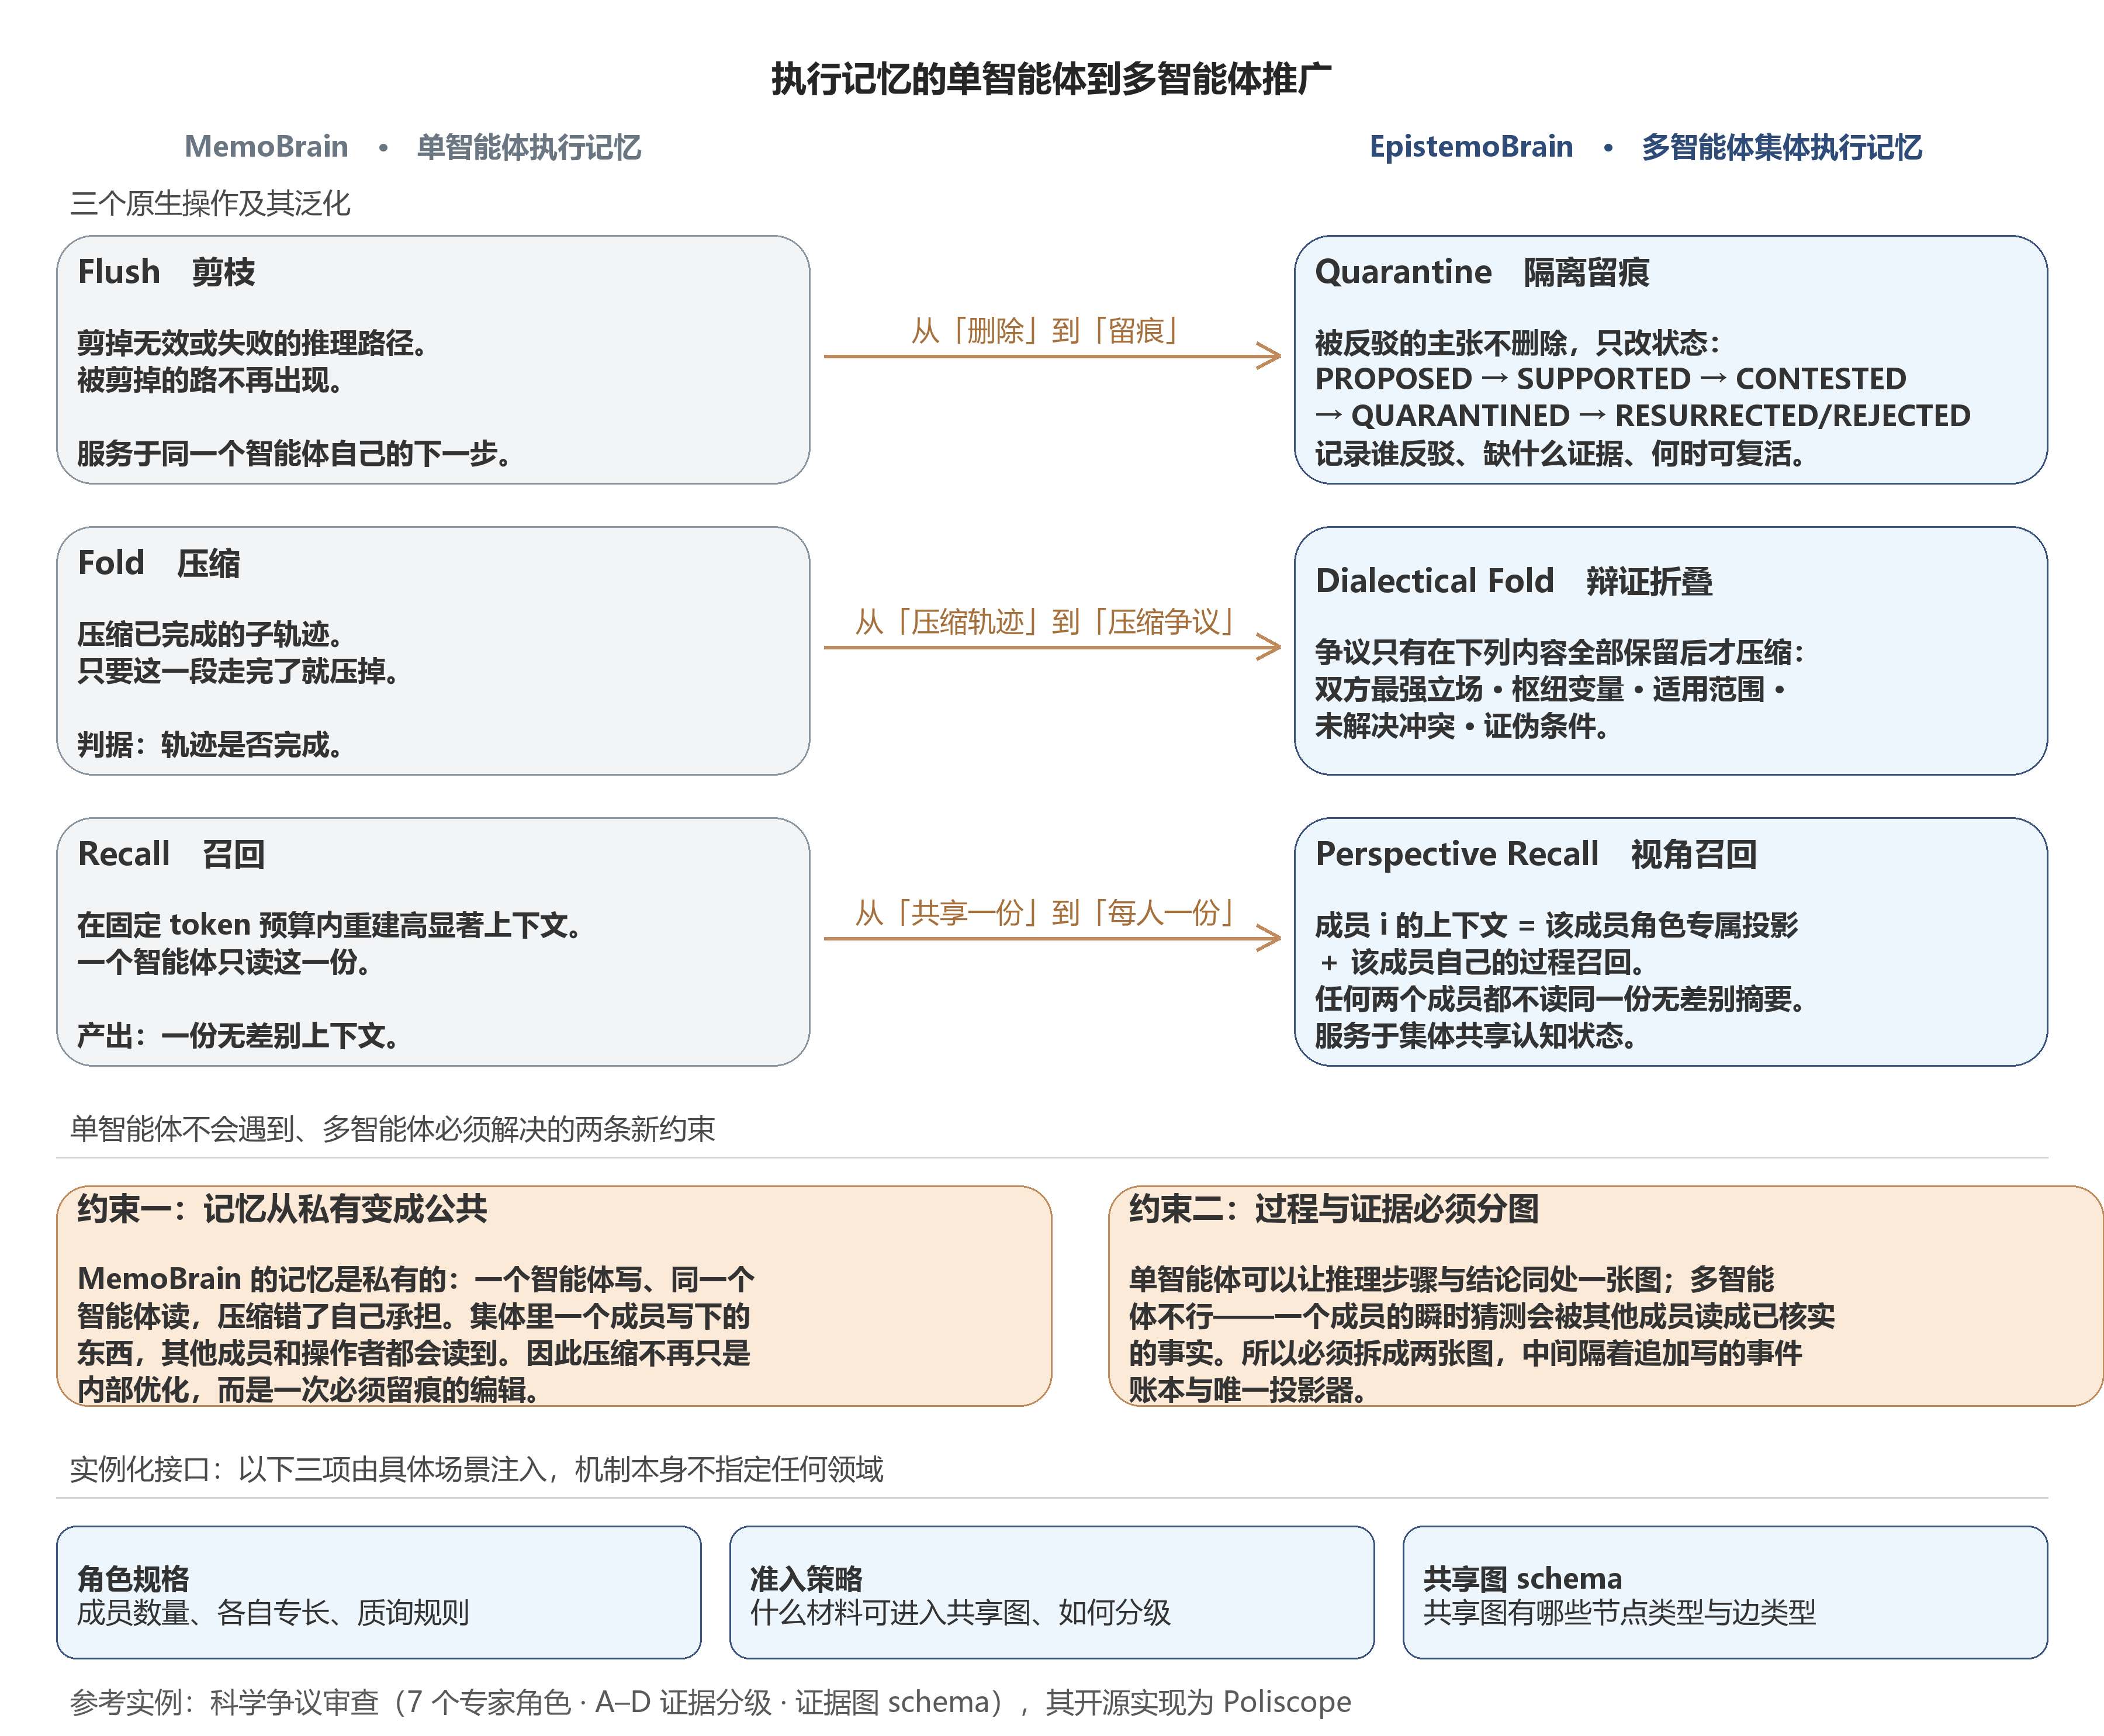
\includegraphics[width=\linewidth]{figures/memobrain-generalization.png}
\caption{执行记忆从单智能体到多智能体的推广。左列为 MemoBrain 的三个原生操作及其单智能体语义，右列为泛化后的操作与多智能体语义，中列标注推动这次转化的判据变化。中部两条约束只在多智能体场景出现：记忆由私有变为公共，过程与证据必须分图。底部为实例化接口——机制本身不指定领域，角色规格、准入策略与共享图 schema 由具体场景注入；科学争议审查是本文使用的参考实例，Poliscope 是它的开源实现。}
\label{fig:generalization}
\end{figure}

\subsection{适配：从单智能体记忆到议会的决策框架}

换的不只是调用方。MemoBrain 原本针对的是「一个 Agent、一个明确目标、逐步淘汰错误路线并保留正确推理骨架」；而议会面对的是「多个科学家围绕一个存在争议、可能没有唯一答案的问题长期协作与对抗」。两者之间有三个本质区别。

\begin{enumerate}[leftmargin=1.6em, itemsep=4pt]
\item \textbf{科研中的「失败观点」可能非常重要。}普通任务里，一条被证明无效的推理路线可以 \code{Flush}；但在科研中，一个当前不被支持的观点可能是有价值的少数派假设、在特殊人群中成立的边界条件、暂时缺少数据的理论解释，或以后会被新证据复活的研究方向。所以不能简单删除。
\item \textbf{科研争议不能被压缩成单一摘要。}普通 \code{Fold} 会把一段辩论总结成「多数证据支持 X」，而这恰恰丢失了最重要的信息：哪些研究不支持 X、不支持的原因是什么、样本或测量口径有什么差异、少数意见在哪些条件下可能成立。压缩一旦消灭异议，系统就会产生\textbf{共识幻觉}。
\item \textbf{不同的科学家需要不同的记忆视图。}因果推断专家要先看到识别策略、混杂变量、反向因果与自然实验；测量专家要先看到变量操作化、量表效度、数据来源与构念漂移。如果所有席位读取完全相同的压缩上下文，多智能体很快就会观点同质化。
\end{enumerate}

这三个区别决定了 EpistemoBrain 相对 MemoBrain 的\textbf{五个扩展}——它们不是功能堆叠，而是依次咬合的：集体记忆要留住争议，留住争议才谈得上识别盲点，识别出盲点才知道该调度谁。

\begin{table}[ht]
\centering\small
\caption{EpistemoBrain 相对 MemoBrain 的五个扩展}
\label{tab:extend}
\begin{tabularx}{\linewidth}{@{}L{2.9cm} L{3.1cm} X@{}}
\toprule
\rowcolor{accent}
\tblhead 扩展 & \tblhead 对应操作 & \tblhead 解决的区别 \\
\midrule
异议保真压缩 & \code{Dialectical Fold} & 争议须在双方最强立场、枢纽变量与证伪条件全部保留之后才压缩（区别 2）\\
证据隔离 & \code{Quarantine} & 被反驳的主张不删除，保留反驳者、缺失证据与复活条件（区别 1）\\
认知分叉 & \code{Fork} / \code{Merge} / \code{Resurrect} & 证据无法区分解释时保留平行路径；新证据满足条件时复活旧假设（区别 1）\\
角色化召回 & \code{Perspective Recall} & 按 \code{Context\_i = ProcessRecall\_i + EvidenceProjection\_i} 计算，七席读到的不是同一份摘要（区别 3）\\
盲点驱动调度 & 盲点悬赏与认识论路由 & 由证据图暴露的缺口决定下一步查什么、由谁查（第 5.3 节）\\
\bottomrule
\end{tabularx}
\end{table}

适配的落点是三层记忆的重新划分（第 5.1 节）：第一层 \code{Private Brain} 直接复用 MemoBrain 的 \code{init\_memory()}、\code{memorize()}、\code{recall()}、token 预算控制与轨迹 Fold，只服务该席位自己，不被其他席位读取；第二层\textbf{集体执行记忆}是本项目的主要创新，它不存聊天记录，只存结构化的认知事件——谁提出了什么、谁攻击了什么、哪些争议尚未解决；第三层争议证据地图则完全移出记忆层，交给双图治理（第 6 章）。记忆层对证据图\emph{没有任何写入权}。

适配的收益是双向的。一方面，议会由此获得了在有限预算内维持长程一致性的机制；另一方面，「记忆由私有变为公共」这条新约束反过来塑造了议会本身的形态——正因为一次压缩的结果会被没写过它的同伴读到，压缩才必须留痕，「过程与证据分图」才成为不可省略的架构决策，而不是可选的工程优化。

\subsection{三根支柱}

整套方法由三根支柱构成，分别对应「谁在研究」「靠什么记得」「什么算证据」。

\begin{enumerate}[leftmargin=1.6em, itemsep=5pt]
\item \textbf{集体协议（Collective Protocol）}回答「谁在研究」。Poliscope 在这一层填入的取值是七人科学议会：七个固定角色各有独立规格、私人状态、私人记忆与证据排序权重，按八阶段协议用结构化动作互相质询。多视角不靠人多，靠每个视角被制度化地挑战。详见第 4 章。
\item \textbf{EpistemoBrain（记忆内核）}回答「靠什么记得」。它把 MemoBrain 的单智能体执行记忆推广到多智能体，管理私人记忆、集体执行记忆与证据图三层，并重新定义三个压缩操作。三层之间形成「过程产生证据、证据暴露盲点、盲点驱动下一轮调查」的闭环——集体记忆不是存档柜，它参与决定下一轮查什么。详见本章「方法定位」与「适配」两节，以及第 5 章。
\item \textbf{双图证据治理（Dual-Graph Governance）}回答「什么算证据」。过程图与证据图物理分离，中间隔着追加写的事件账本、六阶段证据门和唯一投影器。详见第 6、7 章。
\end{enumerate}

\subsection{一次研究的认识论循环}

三根支柱在一次真实任务中串成一条八阶段循环（图~\ref{fig:loop}）。每个阶段都对应一个它专门防止的失败：预承诺防锚定，专业取证防空谈，证据交换防重复阅读，交叉质询防隐藏假设，盲点悬赏把无人触碰的缺口显式化，联合建模防多数票冒充共识，最终复判防信念漂移后无人记账，报告阶段只做组装、不再产生新判断。

\begin{figure}[ht]
\centering
\resizebox{\linewidth}{!}{%
\begin{tikzpicture}[node distance=1.0mm and 3.5mm]
  \node[nda] (p1) {1 独立预承诺};
  \node[nd, right=of p1] (p2) {2 专业取证};
  \node[nd, right=of p2] (p3) {3 证据交换};
  \node[nd, right=of p3] (p4) {4 交叉质询};
  \node[nda, below=of p4] (p5) {5 盲点悬赏};
  \node[nd, left=of p5] (p6) {6 联合建模};
  \node[nd, left=of p6] (p7) {7 最终复判};
  \node[ndd, left=of p7] (p8) {8 报告组装};
  \draw[flow] (p1)--(p2); \draw[flow] (p2)--(p3); \draw[flow] (p3)--(p4);
  \draw[flow] (p4)--(p5); \draw[flow] (p5)--(p6); \draw[flow] (p6)--(p7); \draw[flow] (p7)--(p8);
  \draw[flowg] (p5.south) to[bend right=22] node[lbl,pos=0.5]{缺口生成新调查任务} (p2.south);
\end{tikzpicture}}
\caption{EpistemoBrain 认识论循环：蓝色为两个「判断封存」关键点；第 5 阶段的盲点可回流到第 2 阶段形成增量调查。}
\label{fig:loop}
\end{figure}

\subsection{三条认识论硬约束}

\begin{mechbox}
\boxtag{\color{ink2}不投票}
禁止以多数投票裁决科研真理。即使多数席位支持，只要存在未解决的致命质询或缺乏证据引用，共识就被阻断；最终输出必须同时写出多数判断、具名异议、真正分歧点与解决分歧所需证据（第 4.4 节）。
\end{mechbox}

\begin{mechbox}
\boxtag{\color{ink2}不匿名删除异议}
被反驳、隔离或折叠的观点不做物理删除，只改状态并保留谱系；辩证折叠要求正反双方字段齐备，缺一方就拒绝折叠（第 6.7 节）。
\end{mechbox}

\begin{mechbox}
\boxtag{\color{ink2}不把过程当证据}
任何参与成员都没有证据图写权限；正式修改先写事件账本，由唯一投影器过证据门后落图。这条约束在数据库角色权限层强制，而非依赖代码自律（第 6.5、11.7 节）。
\end{mechbox}

\subsection{与两条主流路线的边界}

Deep Research 优化「读得全」，固定多智能体辩论优化「吵得充分」，EpistemoBrain 优化「被质疑过的结论仍然可追溯」。表~\ref{tab:compare} 给出机制层面的对照，后文每一行都有对应章节落地。

\begin{table}[ht]
\centering\small
\caption{EpistemoBrain 与两类常见研究智能体的机制对照}
\label{tab:compare}
\begin{tabularx}{\linewidth}{@{}L{2.5cm} XXX@{}}
\toprule
\rowcolor{accent}
\tblhead 维度 & \tblhead Deep Research & \tblhead 固定多智能体辩论 & \tblhead EpistemoBrain \\
\midrule
多视角来源 & 单 Agent 换提示词 & 多 Agent 自由发言 & 7 席独立角色规格，结构化动作质询 \\
异议去向 & 并入总结 & 多数意见胜出 & 具名异议证书，永久留图 \\
记忆机制 & 上下文窗口 & 彼此独立、无共享 & 三层记忆，集体记忆调度下一轮 \\
证据标准 & 引用存在即可 & 引用存在即可 & 六阶段证据门 + 因果越级拦截 \\
证据写权限 & 无此概念 & 无此概念 & 数据库层唯一投影器 \\
最终产物 & 流畅综述 & 辩论记录 & 结论与局限并排的可审计证据地图 \\
\bottomrule
\end{tabularx}
\end{table}

% ===================== 第 3 章 =====================
\section{系统架构总览}

\subsection{模块化单体：一个进程内的清晰边界}

Poliscope 采用模块化单体加异步 Worker，首版不做微服务拆分。这是刻意的范围控制：MVP 只需要证明「这套组织结构比普通研究智能体更能发现高价值盲点」，拆分服务对此没有贡献，反而会引入分布式一致性问题。模块边界在代码层强制执行——跨模块只允许通过明确的 Pydantic 契约与应用服务通信，不能直接操作对方的数据表。

\begin{table}[ht]
\centering\small
\caption{14 个内部包的职责划分（\code{packages/}）}
\label{tab:modules}
\begin{tabularx}{\linewidth}{@{}L{3.1cm}X@{}}
\toprule
\rowcolor{accent}
\tblhead 模块 & \tblhead 职责 \\
\midrule
\code{kernel}      & 冻结契约、数据库会话、配置与权限常量；被所有模块依赖，自身不依赖业务模块 \\
\code{council}     & 七席位规格、结构化动作、八阶段注册表、席位与网关的桥接 \\
\code{epistemo}    & 编排器、显式状态机、预算追踪、停止条件、断点恢复 \\
\code{memory}      & MemoBrain 适配器、席位私有记忆、过程图与折叠 \\
\code{evidence}    & 事件账本、证据门、图投影器、谱系、独立性、辩证折叠 \\
\code{papers}      & 查询规划、多源候选发现、规范化、全文解析、发现抽取 \\
\code{models}      & 统一模型网关、成本审计、录制回放、免费体验额度 \\
\code{tools}       & 统一工具网关与四个学术数据源适配器 \\
\code{research}    & 研究契约、主张原子化、任务仓储与应用服务 \\
\code{reports}     & Research Brief 与最终论文组装、Markdown/JSON 双格式、导出脱敏 \\
\code{evaluation}  & ForesightBlindspot 语料、基线/消融接线、语义裁判、标注一致性 \\
\code{accounts}    & 注册登录、邮箱验证码、PBKDF2 口令、bearer 会话 \\
\code{knowledge}   & 个人知识库：多格式解析、全文检索、跨任务复用 \\
\code{skills}      & 从 GitHub 安装研究者技能（SKILL.md），按任务注入议会提示词 \\
\bottomrule
\end{tabularx}
\end{table}

应用层四个入口共享同一套后端契约：\code{apps/api}（FastAPI HTTP 层）、\code{apps/worker}（任务认领与议会执行）、\code{apps/web}（React 证据工作台）、\code{apps/cli}（纯 HTTP 客户端）。CLI 被硬性禁止 import 任何 \code{packages}——第二条直连研究服务的路径，就是一条绕过证据门的路径。

\subsection{一次研究的生命周期}

\begin{enumerate}[leftmargin=1.6em, itemsep=3pt]
\item \textbf{建任务。}研究者提交问题、范围、预算与可选的知识库、PDF、技能；系统原子化出建议主张，任务停在 \code{AWAITING\_CLAIM\_CONFIRMATION}，研究者不确认就不开跑。
\item \textbf{确认主张。}研究者勾选要调查的原子主张后任务入队；被放弃的主张标记为 \code{DISCARDED} 而非删除。
\item \textbf{Worker 认领。}用 \code{SELECT ... FOR UPDATE SKIP LOCKED} 从 PostgreSQL 队列认领，多个 Worker 并发安全；崩溃遗留的 \code{RUNNING} 由 \code{recover\_stale\_running} 回收。
\item \textbf{议会执行。}七席乘八阶段在一次数据库事务内跑完，每席经统一网关与模型交互，结构化动作追加进事件账本。
\item \textbf{图投影。}投影器以第二个数据库身份、第二个事务消费账本事件，过证据门后写入证据图。
\item \textbf{报告。}终态时从证据图、账本与任务行组装 Research Brief 和最终论文，报告阶段不调用模型产生新判断。
\end{enumerate}

\subsection{架构全景}

\begin{figure}[ht]
\centering
\resizebox{\linewidth}{!}{%
\begin{tikzpicture}[node distance=2.6mm and 6mm]
  \node[ndd, minimum width=30mm] (web) {Web 工作台 / CLI};
  \node[nd, below=of web, minimum width=30mm] (api) {FastAPI 应用层（apps/api）};
  \node[nda, below=of api, minimum width=30mm] (worker) {Worker：七席 × 八阶段议会};
  % left rail
  \node[nd, left=11mm of worker, minimum width=24mm] (mg) {模型网关\newline\tiny 分层模型 · 审计};
  \node[nd, below=of mg, minimum width=24mm] (tg) {工具网关\newline\tiny 四大学术源};
  % center chain
  \node[nd, below=of worker, minimum width=30mm] (ledger) {科学事件账本（追加写 · 幂等）};
  \node[nd, below=of ledger, minimum width=30mm] (gate) {六阶段证据门};
  \node[ndd, below=of gate, minimum width=30mm] (proj) {Graph Projector（唯一写入者）};
  \node[nda, below=of proj, minimum width=30mm] (graph) {证据图（10 类节点 / 12 类边）};
  % right rail
  \node[nd, right=11mm of ledger, minimum width=24mm] (proc) {过程图 + 三层记忆\newline\tiny Flush/Fold/Recall};
  \node[nd, below=of proc, minimum width=24mm] (bs) {盲点悬赏\newline\tiny 回流再调查};
  \draw[flow] (web)--(api); \draw[flow] (api)--(worker);
  \draw[flow] (worker)--(ledger); \draw[flow] (ledger)--(gate);
  \draw[flow] (gate)--(proj); \draw[flow] (proj)--(graph);
  \draw[flowg] (worker)--(mg); \draw[flowg] (worker)--(tg);
  \draw[flowg] (worker)--(proc);
  \draw[flow] (graph)--(bs); \draw[flowg] (bs.north) to[bend left=18] (worker.east);
\end{tikzpicture}}
\caption{系统架构：应用、议会、账本、证据门、投影器构成主干；模型/工具网关是唯一外部出口；过程图与证据图分居两侧，盲点回流驱动增量调查。}
\label{fig:arch}
\end{figure}

\subsection{两个事务、两个数据库身份}

「投影器是证据图唯一写入者」如果只写在文档里，就只是愿望。Poliscope 在 PostgreSQL 角色层把它变成硬事实：

\begin{itemize}[leftmargin=1.6em, itemsep=3pt]
\item 应用身份 \code{poliscope\_app} 可以追加账本、读取证据图，但对证据图表没有 \code{INSERT/UPDATE/TRUNCATE} 权限；
\item 投影器身份 \code{poliscope\_projector} 可以写图、推进事件状态，但不能改写既有事件 payload，且没有 \code{DELETE}（会话删除是唯一的迁移级例外，见第 9.7 节）；
\item 两个身份都不能 \code{TRUNCATE}。
\end{itemize}

Worker 因此把一次运行拆成两个事务：议会事务以应用身份提交动作，投影事务以投影器身份落图。集成测试 \code{test\_graph\_write\_isolation.py} 逐条断言应用身份写图会被数据库直接拒绝——这不是代码自律，是数据库事实。

\subsection{为什么队列建在 PostgreSQL 而不是 Redis}

任务认领与状态更新必须在同一个事务里完成，Worker 崩溃时行锁随事务自动释放，不会留下「谁在跑」的悬空状态。引入 Redis 等于多一个可能与数据库不一致的真相来源，而首版没有任何组件需要 Redis 做缓存或广播。少一个服务，就少一类故障与一份运维成本。

% ===================== 第 4 章 =====================
\section{七人科学议会}

\subsection{七个固定席位}

每个正式研究任务中，七个席位全程参与，定义在 \code{packages/council/contracts.py} 的 \code{Seat} 枚举。席位不是可选项标签，而是各自拥有独立角色规格（\code{roles.py::ROLE\_SPECS}）、独立私人记忆（agent id 为 \code{\{task\_id\}:\{seat\}}，没有任何代码读取他人 id）和不同证据排序权重（\code{packages/memory/projection.py}）。这三项差异都有测试锁定——历史上曾出现五个席位共用一份空权重、在唯一用于区分它们的维度上互为复制品的事故。

\begin{table}[ht]
\centering\small
\caption{七个席位与其质询重心}
\label{tab:seats}
\begin{tabularx}{\linewidth}{@{}L{4.0cm} X@{}}
\toprule
\rowcolor{accent}
\tblhead 席位（标识） & \tblhead 质询重心 \\
\midrule
理论建构者 \seat{theory\_builder}            & 竞争理论、机制链条、风险预测是否成立 \\
因果推断专家 \seat{causal\_scientist}        & 混杂、反向因果、选择偏差、识别策略 \\
测量与构念专家 \seat{measurement\_scientist} & 构念与操作化的距离、自报告偏差、测量不变性 \\
统计与复现专家 \seat{replication\_scientist} & 功效、精度、多重比较、复现史 \\
边界与情境专家 \seat{boundary\_scientist}    & 适用范围、异质性、外推条件 \\
对抗性证伪者 \seat{adversarial\_falsifier}   & 攻击结论的最强版本，主动寻找反例与零结果 \\
证据与溯源审计员 \seat{evidence\_auditor}    & 来源锚点、引用蕴含、证据独立性 \\
\bottomrule
\end{tabularx}
\end{table}

议会之上没有第八名科学家：调度、记录与组装由编排层承担，它\textbf{无投票权}，不代表任何学术立场；\code{EpistemoBrain} 则位于编排层之下的记忆层，只负责记忆的压缩与重建，同样不参与任何裁决。七席共享同一套运行框架（\code{deliberation.py} 中唯一的 \code{GatewayDeliberator} 类服务全部席位）与同一个工具缓存，既满足「不复制七套业务代码、不部署七个服务」，又保住席位之间的独立性。

\subsection{八阶段协议}

阶段顺序由 \code{packages/epistemo/contracts.py} 的 \code{PHASE\_SEQUENCE} 冻结，状态机只允许顺序前进（第 9.1 节）。

\begin{enumerate}[leftmargin=1.6em, itemsep=3pt]
\item \textbf{独立预承诺。}七席在看到他人意见前，分别提交初始判断、置信度、三个最可能的盲点、待补证据与改判条件。预承诺封存后才允许读取，读取后不能补交——后续一致性因此无法来自锚定。
\item \textbf{专业取证。}各席按自身维度提出证据需求，查询规划器合并去重后批量检索（第 8.4 节），驱动搜索的是证据需求矩阵而不是泛泛关键词。
\item \textbf{证据交换。}交换结构化证据（主张、原文片段、研究设计、质量等级、适用边界），不交换完整思维链。
\item \textbf{交叉质询。}目标是暴露隐藏假设而非争胜。被质询方只能回应 \code{DEFEND / REVISE / NARROW / WITHDRAW / DISSENT} 五种动作之一。
\item \textbf{盲点悬赏。}证据图暴露的缺口生成盲点候选，按「影响 $\times$ 不确定性 $\times$ 可调查性 $\times$ 新颖度 $-$ 成本」打分，广播给七席共同认领。
\item \textbf{联合建模。}把各席结论组合为条件化共识；最强反对或证伪条件缺失时拒绝出共识。进入本阶段前有唯一的人类引导检查点（第 4.5 节）。
\item \textbf{最终复判。}七席再次独立判断，记录信念更新轨迹；仍持异议的席位获得具名异议证书。复判只遍历实际参与的席位，不为缺席者伪造判断（这条由评测基线的一次事故促成，见第 10.5 节）。
\item \textbf{报告组装。}从图与账本组装产物，本身不产生新的模型判断。
\end{enumerate}

一个席位失败不会拖垮任务：失败被记为该轮 \code{SEAT\_UNAVAILABLE} 事件与一个未填槽位，其余席位继续，任务最终以 \code{COMPLETED\_WITH\_GAPS} 收尾，缺席者在报告局限一节逐条点名（第 9.4 节）。

\subsection{结构化科研动作：科学家能说什么是被限定的}

科学家不能向账本写自由发言，只能提交八类结构化动作；收到质询后，回应动作再收窄为五类。

\begin{center}\small
\begin{tcolorbox}[colback=panel, colframe=linegray, boxrule=0.6pt, arc=2pt, left=8pt,right=8pt,top=6pt,bottom=6pt, fontupper=\ttfamily]
主动作：PROPOSE\quad SUPPORT\quad CHALLENGE\quad QUALIFY\quad FORK\quad REQUEST\quad REVISE\quad DISSENT\\[3pt]
应答：DEFEND\quad REVISE\quad NARROW\quad WITHDRAW\quad DISSENT
\end{tcolorbox}
\end{center}

每个动作必须携带 actor、target、statement、\code{evidence\_refs}、confidence、\code{falsification\_condition}、novelty。校验器（\code{council/actions.py}）会拒绝：没有目标节点的泛泛评论、没有来源的事实主张、与既有内容高度重复的观点、只有「我同意」而无新增信息的发言、以及说不出如何被推翻的绝对断言。动作词汇表本身就是一份「科研讨论该长什么样」的形式化约束。

\subsection{禁止多数投票：共识如何被阻断}

在 \code{evaluate\_consensus} 中，即使多数席位投出 \code{SUPPORT}，只要存在未解决的致命质询（\code{has\_unresolved\_fatal\_challenge}）或证据引用为空，共识状态就是 \code{BLOCKED}。联合建模处理器在最强反对与证伪条件缺失时同样拒绝产出共识。因此最终输出不是票数，而是四段式结构：

\begin{mechbox}
\textbf{多数判断}：存在小幅、条件性的影响。\\
\textbf{少数异议}：现有研究不足以排除反向因果。\\
\textbf{真正分歧}：纵向时间顺序能否被视为充分的因果证据。\\
\textbf{解决分歧所需证据}：带平台日志与基线心理健康控制的预注册纵向研究。
\end{mechbox}

\subsection{人类方向性引导检查点}

盲点悬赏结束、联合建模开始之前，任务进入 \code{AWAITING\_COUNCIL\_INPUT}：研究者可以查看七席此刻的立场（预承诺、置信度、已提质询），提交一段方向性备注，也可以明确留空。这个检查点有四条边界，保证它不违反「禁止投票」：它是单一研究者的调度性输入而非票数；只影响下一轮重点讨论哪些冲突；不改变任何证据门判定；不会作为证据进入任何正式节点。备注在联合建模提示词中以独立、显式标注的文本块注入（如「[研究者方向性备注，非科学判断]：……」）。

研究者离开页面不会卡住任务：宽限期默认 900 秒（15 分钟；环境变量全名见附录 A.4，下限 30 秒），届满自动以「无干预」回到队列续跑。实现横跨状态枚举、\code{CouncilCheckpoint.guidance} 字段、预览与引导两个 API 端点（\code{council-preview}、\code{council-guidance}）、CLI 子命令与前端 \code{CheckpointGate.tsx}。

% ===================== 第 5 章 =====================
\section{三层记忆与 MemoBrain 适配}

\subsection{记忆是公共认知层，不是私有缓存}

这是多智能体推广带来的第一处变化。MemoBrain 的记忆是\textbf{私有}的：一个智能体写、同一个智能体读，压缩错了自己承担后果。议会里的记忆是\textbf{公共}的：一个席位写下的东西会被其他六个席位和研究者读到，所以压缩不再只是内部优化，而是一次\textbf{必须留痕的编辑}——这正是 Flush 要变成 Quarantine、Fold 要变成 Dialectical Fold 的原因。

Poliscope 把「记得什么」分成三层，各层回答不同的问题，也遵守不同的写入规则。

\begin{table}[ht]
\centering\small
\caption{三层记忆的分工}
\label{tab:memory}
\begin{tabularx}{\linewidth}{@{}L{2.8cm} L{3.2cm} X@{}}
\toprule
\rowcolor{accent}
\tblhead 层 & \tblhead 回答的问题 & \tblhead 内容与规则 \\
\midrule
私人记忆 Private Memory & 这位科学家怎么走到这一步 & 个人探索轨迹、工具记录、未验证猜想；只服务本人，他人不可读 \\
集体执行记忆 Collective MemoBrain & 共同体研究到哪一步、下一步查什么 & 结构化认知事件：谁提出什么、谁挑战谁、哪些争议悬着、哪些缺口没人碰；参与调度下一轮 \\
证据图 Evidence Graph & 我们目前对问题知道什么 & 只存经过审计的正式知识，唯一投影器可写（第 6 章） \\
\bottomrule
\end{tabularx}
\end{table}

三层之间是闭环而非堆叠：过程产生证据，证据暴露盲点，盲点作为新任务回灌私人记忆，驱动下一轮调查。集体记忆在这个闭环里承担执行控制职责——是证据状态决定下一步派谁查什么，而不是主持人按固定台本点名。

\subsection{MemoBrain 适配：小接口、不改上游}

MemoBrain 是外部方法基座（\code{github.com/qhjqhj00/MemoBrain}），集成前已核验许可证。Poliscope 通过 \code{MemoBrainAdapter} 对接，不修改上游源码，首版适配面刻意压到五个方法：

\begin{lstlisting}[language=ps]
init_private_memory(agent_id, task)
memorize_episode(agent_id, episode)
recall_private(agent_id, token_budget)
save_snapshot(agent_id)
load_snapshot(agent_id)
\end{lstlisting}

\begin{honestbox}
\boxtag{\color{warnamber}实现现状（不夸大）}
当前 \code{create\_memory\_adapter()} 返回的是 \code{InMemoryMemoryAdapter} 内存替身，过程图的 Flush/Fold/Recall 为简化实现，尚未真正导入上游 MemoBrain 代码。接口与边界已冻结，替换为真实实现不需要改动议会与证据层。这是首版明确保留项，详见第 12 章。
\end{honestbox}

\subsection{席位私有记忆的隔离规则}

隔离只靠一条规则做到位：agent id 由任务 id 与席位拼接，代码中不存在读取「另一个席位 id」的路径。于是同一任务的两席互相看不到对方的召回内容，同一席位也不会把 A 任务的记忆带进 B 任务。\code{CouncilMemory} 负责播种任务、记录 episode、按席召回与快照恢复。

\textbf{召回预算刻意设得很小：每席 800 字符}（\code{DEFAULT\_RECALL\_BUDGET}）。召回内容与证据投影竞争同一份上下文，它的目标是保住科研骨架而非重放完整转录——当前任务、已确认发现、活跃盲点、未决质询、少数异议、下一步证据需求，这六项在 800 字符内足以保全，而后面每一轮的提示词不会被不断增长的转录撑爆。

\subsection{过程记忆的 Fold：保骨架，不保字数}

\code{packages/memory/fold.py} 的 \code{fold\_process} 只接受过程图快照；任何试图折叠证据图节点的调用直接抛 \code{GraphBoundaryViolation}。压缩按任务、工具调用、决策三类节点进行，压缩前必须通过六项骨架保留校验：

\begin{center}
\begin{tcolorbox}[colback=panel, colframe=linegray, boxrule=0.6pt, arc=2pt, fontupper=\sffamily\small]
当前任务\enspace·\enspace 已确认 Finding\enspace·\enspace 活跃 Blindspot\enspace·\enspace 未解决质询\enspace·\enspace 少数异议\enspace·\enspace 下一步证据需求
\end{tcolorbox}
\end{center}

六项有一项丢失，折叠结果即标记为 rejected、原快照保留。

这里有一条容易忽略的分界：普通 Fold 只能作用于过程图。证据图只允许保留异议的辩证折叠（Dialectical Fold，第 6.7 节），两条折叠路径不可混用——它们保护的东西不同，一条守着上下文预算，另一条守着异议本身。

\subsection{Perspective Recall：同一份证据，不同的排序}

不同席位面对同一份证据快照时，按各自的 \code{evidence\_sort\_weights} 得到不同排序：因果专家先看到混杂与反向因果攻击，测量专家先看到构念冲突与测量不变性质疑。形式化地：
\[
\text{Context}_i = \text{ProcessRecall}_i + \text{EvidenceProjection}_i
\]
这同时避开了多智能体两个常见失败：每个 Agent 重复阅读全部材料，以及所有 Agent 最终收敛出相同观点。

去重的是检索成本，不是认知视角。

\subsection{认识论路由：让证据状态调度调查}

证据图发现缺口后，路由依次执行：生成盲点候选并打分 $\rightarrow$ 分派给全部七席（每席一个固定角色角度） $\rightarrow$ 分配角色化上下文 $\rightarrow$ 执行检索验证 $\rightarrow$ 结果写回集体记忆 $\rightarrow$ 重算认知前沿。注意这不是「选一个最强科学家单干」，也不是「一人认领一条」：七席全程在场，同一条盲点由七个角色角度同时调查，分工表在盲点悬赏轮\textbf{确定性}生成——同样的输入重跑一遍，得到的是同一张表。

% ===================== 第 6 章 =====================
\section{双图治理与科学事件账本}

\subsection{为什么必须是两张图}

过程图回答「科学家是怎样完成这次研究的」，证据图回答「我们目前对这个问题知道什么」。合并成一张图会同时引发五类问题：工具调用步骤与学术证据混杂；Agent 的中间猜想被误读为事实；压缩推理过程时误删证据；一篇论文里的多个发现无法精确表示；界面无法清晰呈现争议结构。因此两张图在存储、权限与折叠规则上全部隔离。

\begin{itemize}[leftmargin=1.6em, itemsep=3pt]
\item \textbf{过程图 Process Graph}：任务、工具调用、失败路线、质询与决策，由记忆层管理，允许普通 Flush/Fold/Recall，节点永不自动成为正式证据。
\item \textbf{证据图 Evidence Graph}：10 类正式节点、12 类正式边（速查表见附录 A），只存经过审计的知识，只有图投影器能写。
\end{itemize}

\subsection{科学事件账本：一切正式修改的唯一入口}

七名科学家不得直接写证据图，所有正式修改必须先写入 \code{packages/evidence/sql\_ledger.py} 的 \code{SqlEventLedger}。账本设计了四条性质。

\begin{enumerate}[leftmargin=1.6em, itemsep=3pt]
\item \textbf{幂等、可重放。}唯一约束 \code{uq\_event\_idempotency} 加全序 \code{sequence}（\code{coalesce(max(sequence),0)+1}）。同一批事件重放任意次，结果相同。
\item \textbf{冲突可见。}同一幂等键提交不同 payload 时抛 \code{EventConflict}，任何改写历史的尝试都无法静默通过。
\item \textbf{并发串行化。}PostgreSQL 事务级咨询锁（\code{pg\_advisory\_xact\_lock}）保证并发提交不乱序。
\item \textbf{过程事件不升级。}仅过程类事件允许 \code{on\_conflict="skip"}，正式事件不享受此通道。
\end{enumerate}

幂等键由阶段、席位与位置派生（\code{PhaseContext.key()}，含超长查询的哈希折叠——这是修复过真实生产事故的细节：把 \code{uuid4()} 放进 payload 的轮次会在重放时与自己的幂等键冲突，现有测试专门盯防这一回退）。

\subsection{图投影器：证据图的唯一写入者}

\code{packages/evidence/sql\_projector.py} 的 \code{SqlGraphProjector} 顺序消费账本事件，机制包括：节点事件类型白名单（过程事件直接拒绝）；\code{node\_id\_for} 保证节点跨重放 id 稳定；写入边时对悬空目标抛 \code{ProjectionError}；checkpoint 单调不回退。投影器与应用身份的数据库权限划分已在第 3.4 节给出，此处不再重复。

\subsection{双图双向联动}

\begin{figure}[ht]
\centering
\resizebox{\linewidth}{!}{%
\begin{tikzpicture}[node distance=3mm and 10mm]
  \node[nd, minimum width=34mm, minimum height=12mm] (proc) {\textbf{过程图}\newline\tiny 思考 · 检索 · 失败路线 · 质询};
  \node[nda, right=of proc, minimum width=30mm, minimum height=12mm] (led) {\textbf{事件账本 + 证据门}\newline\tiny 追加写 · 幂等 · 六阶段审计};
  \node[ndd, right=of led, minimum width=34mm, minimum height=12mm] (ev) {\textbf{证据图}\newline\tiny 主张 · 发现 · 来源 · 盲点};
  \draw[flow] (proc.north) to[bend left=20] node[lbl,above]{① 结构化事件送审} (led.north);
  \draw[flow] (led.north) to[bend left=20] node[lbl,above]{② 过审后投影落图} (ev.north);
  \draw[flow] (ev.south) to[bend left=20] node[lbl,below]{③ 缺口生成盲点与新任务} (led.south);
  \draw[flowg] (led.south) to[bend left=20] node[lbl,below]{④ 新任务回灌私人记忆} (proc.south);
\end{tikzpicture}}
\caption{双图联动：正向通道把过程提炼为证据，回流通道把证据缺口变成下一轮过程；两个方向都经过账本，没有旁路写入。}
\label{fig:dualgraph}
\end{figure}

\textbf{正向（过程 $\rightarrow$ 证据）}：科学家完成「思考 $\rightarrow$ 检索 $\rightarrow$ 阅读 $\rightarrow$ 抽取发现 $\rightarrow$ 提交动作」整段过程，过程图全程记录，但只有结构化事件进入审计通道。\textbf{回流（证据 $\rightarrow$ 过程）}：证据图发现「支持某主张的七项发现全部来自自报告数据」这类缺口，生成 \code{Blindspot} 与新的调查任务，写入相关席位的私人记忆，开启增量调查。两条路径都经过账本，不存在绕过审计的写入。

\subsection{被反驳的节点淡化，但永不消失}

投影器的 upsert 只改 \code{status}、不删行；辩证折叠要求正反双方字段全部非空，缺字段就拒绝折叠（\code{dialectical\_fold.py}）；异议证书挂在事件本体上，报告组装无法把它「总结没」。前端证据地图遵循同一条规则：被反驳节点淡化显示（dimmed, never hidden）。对应回归测试包括 \code{test\_dissent\_preservation.py} 与 \code{test\_dialectical\_fold.py}。

% ===================== 第 7 章 =====================
\section{证据门、三层审计与证据谱系}

\subsection{六阶段证据门}

每个候选事件在 \code{packages/evidence/gate.py} 的 \code{FullEvidenceGate} 中依次通过六个阶段，前一阶段不通过就不进入下一阶段，审计结论逐行落库。

\begin{table}[ht]
\centering\small
\caption{证据门六个阶段的职责}
\label{tab:gate}
\begin{tabularx}{\linewidth}{@{}L{4.0cm} X@{}}
\toprule
\rowcolor{accent}
\tblhead 阶段 & \tblhead 检查内容 \\
\midrule
SCHEMA              & 字段完整性与类型正确性 \\
DEDUPLICATION       & 与既有对象的语义重复判定，重复即不消耗后续预算 \\
SOURCE              & DOI 解析、标题/作者/年份一致性、撤稿状态 \\
CITATION\_ENTAILMENT& 原文是否真的支持被绑定的主张 \\
METHOD\_QUALITY     & 直接性、设计强度、测量效度、统计精度、可复现性、外部效度 \\
GRAPH\_CONSISTENCY  & 是否制造矛盾节点、重复分叉谱系等图约束破坏 \\
\bottomrule
\end{tabularx}
\end{table}

第六阶段不是恒真空检查：它调用 \code{consistency.py::check\_graph\_consistency()}，所需布尔值来自 \code{SqlGraphConsistencyQuery} 对数据库的真实查询。第三、五阶段读取候选事件自带的元数据，撤稿论文在此被拒。

\subsection{证据分级 A–D：等级不够就进不了结论}

\begin{table}[ht]
\centering\small
\begin{tabularx}{\linewidth}{@{}c L{4.6cm} X@{}}
\toprule
\rowcolor{accent}
\tblhead 等级 & \tblhead 可得性 & \tblhead 处置 \\
\midrule
A & 全文与精确原文可得      & \code{ADMIT}，节点状态 active \\
B & 仅有摘要与可靠元数据    & \code{SOURCE\_ONLY}，节点 provisional，不得单独支撑高置信因果结论 \\
C & 综述中的二手描述        & \code{DISCOVERY\_ONLY}，留账本、不入图 \\
D & 网页或新闻线索          & \code{TOOL\_LEAD\_ONLY}，留账本、不入图 \\
\bottomrule
\end{tabularx}
\end{table}

\begin{honestbox}
\boxtag{\color{warnamber}实事求是：当前管线只产 B 级}
首版取证管线能稳定拿到的是题录与摘要元数据，因此正式发现最高只到 B 级。这不是配置遗漏：在拿不到全文时把证据标成 A 级，等于默许高置信因果结论建立在摘要之上。等级标签是承诺，不是装饰。
\end{honestbox}

\subsection{三层审计：防止六类常见误写}

正式 Finding 必须依次通过来源真实性（\code{source\_verifier.py}）、引用蕴含（\code{citation\_verifier.py}）与方法质量（\code{method\_auditor.py}）三层审计。引用蕴含层专门拦截六类高频误写：引言里的假设被写成实测结果；讨论段的推测被写成实证发现；不显著被写成「没有效应」；相关被升级为因果；子群结果被外推为总体结论；作者未检验的机制被写成已验证机制。

\subsection{因果越级拦截}

\code{CausalUpgradePolicy} 在证据门内专门识别「横截面设计 + 因果主张」的组合，命中即隔离事件并留审计记录。「相关不等于因果」在多数系统里是一句提示语，在这里是一条不可绕过的判定规则。

\subsection{证据谱系：论文数量不等于独立证据数量}

\code{lineage.py} 定义八类证据依赖关系：同一数据集、重叠样本、同一研究团队、预印本与正式版、扩展研究、再分析、引用但无新数据、综述纳入。\code{independence.py} 的 \code{cluster\_evidence} 用并查集把存在依赖的研究聚成独立证据簇——同一实验室的两个不同数据集不合并，但共享同一份数据的六篇论文只算一簇。界面与报告会同时展示论文数与独立证据簇数，两个数字的差距本身就是在向研究者报警。

\subsection{防止共享错误被当成共识的四道防线}

\begin{enumerate}[leftmargin=1.6em, itemsep=3pt]
\item \textbf{盲证据评审。}首轮判断剥离作者、期刊、被引量等声誉信号，只给方法、样本与结果。当前由结构性测试锁定网关不透传声誉字段；主动剥离的轮次处理器属保留项（第 12 章）。
\item \textbf{独立双抽取。}高影响论文由两个不同模型/角色独立抽取后比对。首版未实现，列入路线图。
\item \textbf{来源多样性约束。}当一项主张的全部支持证据来自同一数据集、团队、国家、测量方式或设计时，\code{source\_diversity.py} 自动生成盲点，并禁止给出高置信结论。
\item \textbf{对抗式检索。}\code{adversarial\_retrieval.py} 为每条已确认主张生成六类反向检索意图（反驳、零结果、替代理论、测量批评、复现失败、边界翻转）并发起真实查询；查不到就如实记录尝试次数，不伪造命中。
\end{enumerate}

% ===================== 第 8 章 =====================
\section{token 经济学：七人全程参与如何不烧钱}

七席全程参与天然比单 Agent 昂贵。Poliscope 的选择不是「动态省略席位」——任何一次省略都是在赌这个角色这次用不上，而盲点恰恰长在被省略的视角里。

成本控制的第一层来自 \textbf{EpistemoBrain} 本身。执行记忆的原始收益就是「不让上下文膨胀」：已完成的子轨迹折叠成摘要节点，无效路径不再占窗口，推理骨架始终留在预算内。推广到多智能体之后又添了三条——\textbf{共享检索缓存}合并的是成本而不是视角；\textbf{发言预算}让没有新信息的席位 \code{PASS}；语义去重命中则不触发强推理。剩下的由工程层补齐：八层机制共同作用，表~\ref{tab:cost} 先给全景。

\begin{table}[ht]
\centering\small
\caption{八层成本控制机制与落点}
\label{tab:cost}
\begin{tabularx}{\linewidth}{@{}L{3.4cm} L{3.6cm} X@{}}
\toprule
\rowcolor{accent}
\tblhead 机制 & \tblhead 控制点 & \tblhead 实现位置 \\
\midrule
发言预算       & 每轮每席至多一个主动作、一个质询、一个回应，无新信息即 PASS & 各轮处理器收集逻辑 \\
新颖性门控     & 语义去重命中则不调用强推理、不写集体图 & 证据门 DEDUPLICATION \\
分层模型       & 强判断用强模型，机械操作用轻量模型 & \code{deliberation.py::PHASE\_MODEL\_CLASSES} \\
共享检索缓存   & 七席证据需求合并去重，一篇论文只下载/解析/验证一次 & 查询规划器 + 统一候选池 \\
调用审计       & 每次模型/工具调用记录 token、费用、延迟、重试 & 审计装饰器网关 \\
四维预算       & 时长、费用、工具次数、来源数同时设限，花前检查 & \code{epistemo/budget.py} \\
阶段 deadline  & 整轮 15 分钟、单席重试至多 2 次，超时记缺席不陪跑 & Worker 收集器 \\
召回预算       & 每席召回 800 字符，保骨架不重放转录 & \code{council\_memory.py} \\
\bottomrule
\end{tabularx}
\end{table}

\subsection{分层模型调用：把强模型用在判断上}

\code{PHASE\_MODEL\_CLASSES} 按阶段分配模型档位：预承诺、交叉质询、盲点悬赏、最终复判四个「判断质量决定结果」的阶段使用强推理档；取证、证据交换、联合建模使用中档模型。部署时通过 \code{POLISCOPE\_MODEL\_NAME\_STRONG\_REASONING / \_MEDIUM / \_LIGHTWEIGHT} 分别指定，留空时按「任务自带配置 $\rightarrow$ 部署默认 $\rightarrow$ 轻量兜底」顺序回退。档位与阶段的绑定关系进代码、不进提示词，避免模型自己决定用哪个模型。

\subsection{共享检索缓存：合并的是成本，不是视角}

七席各自提出证据需求后，查询规划器对检索意图做合并去重，检索器批量执行，结果进入统一候选池。同一篇论文的 PDF 只下载一次、文本只解析一次、DOI 只验证一次、元数据统一缓存；各席仍按自己的视角读取不同字段与片段。认知多样性发生在阅读与质询环节，检索环节没有理由为相同关键词付七次钱。

\subsection{每一笔成本都可解释}

所有模型调用经过 \code{AuditedModelGateway} 装饰器，\code{models/audit.py} 把 input/output token、费用、延迟、重试次数与结构化输出修复状态逐笔落库；工具调用由 \code{AuditedToolGateway} 同等待遇。

研究者在界面上能看到钱花在了哪个阶段、哪个席位。成本数据本身也是第 10 章「每个有效盲点成本」指标的来源。

\subsection{四维预算：耗尽时报告缺口，不伪造完整}

\code{BudgetTracker} 同时追踪总时长、模型费用、工具调用数与来源数四个维度，每个消费者在扣减前检查剩余。

预算耗尽抛 \code{BudgetExhausted}，任务以 \code{COMPLETED\_WITH\_GAPS} 收尾，未完成的证据槽位逐条列出。预算不足是一种需要被看见的系统状态，不是让模型悄悄写满结论的理由。

\subsection{阶段级 deadline 与超时回退}

整轮收集默认 15 分钟上限，单席至多重试 2 次；模型网关自身采用「流式 240 秒 $\rightarrow$ 非流式 300 秒」的回退链，结构化输出修复至多 1 次，修复失败的输出被隔离，绝不写入正式图。

一个席位挂起时，其余六席的工作不被绑架。

\subsection{免费体验与 BYOK：成本选择权在研究者}

系统同时支持部署方承担费用与研究者自带密钥（BYOK，任务级 \code{model\_config}）。免费体验通道走 \textbf{DeepSeek}（\code{deepseek-v4-flash}），\textbf{每个账户限用一次}（\code{FREE\_TRIAL\_LIMIT = 1}），在确认主张时以单行原子操作扣减，并发请求无法双重消耗额度。密钥只存服务器与任务行，任何读取端点都不回显，不进仓库、日志与前端；研究者自己的端点在保存前必须通过一次 10 秒连通性探测，误把控制台门户当 API 端点的情况会被当场拒绝并给出修正提示。

额度按账户计，因此「注销后重新注册」是一条反复消耗体验额度的路径——注销会释放账号占用的邮箱，而邮箱是注册的唯一凭证。系统的选择是\textbf{不提供注销账户功能}：账号是永久的，想换个身份的研究者可以在这里改用户名或改密码。邮箱验证把注册门槛提到「需要一个真实邮箱」，配合账号不可注销，把这条路径基本封住（换一个全新邮箱重新注册仍然可行，这是邮箱注册制本身的边界，不是本系统的漏洞）。

% ===================== 第 9 章 =====================
\section{可靠性工程：状态机、续跑与降级}

\subsection{显式状态机：跳转非法即报错}

\code{packages/epistemo/state\_machine.py} 的 \code{TaskStateMachine} 冻结全部合法状态与转移，阶段推进只允许走到下一阶段，跳步抛 \code{InvalidTransition}。任务主状态机如图~\ref{fig:states}。

\begin{figure}[ht]
\centering
\resizebox{\linewidth}{!}{%
\begin{tikzpicture}[node distance=2.2mm and 5mm]
  \node[nd] (a) {待确认主张};
  \node[nd, right=of a] (q) {QUEUED};
  \node[nda, right=of q] (r) {RUNNING};
  \node[nd, below=7mm of q] (w) {等待人类引导\newline\tiny AWAITING\_COUNCIL\_INPUT};
  \node[ndd, right=12mm of r] (t1) {COMPLETED};
  \node[nd, below=3mm of t1] (t2) {COMPLETED\_WITH\_GAPS};
  \node[nd, below=3mm of t2] (t3) {FAILED / CANCELLED};
  \draw[flow] (a)--(q); \draw[flow] (q)--(r);
  \draw[flow] (r)--(w); \draw[flow] (w)--(q);
  \draw[flow] (r)--(t1); \draw[flow] (r)--(t2); \draw[flow] (r)--(t3);
\end{tikzpicture}}
\caption{任务主状态机：人类引导检查点回到队列续跑；终态三分支区分完整完成、带缺口完成与失败/取消。}
\label{fig:states}
\end{figure}

\subsection{事务语义：一次议会跑在一个未提交事务里}

Worker 的 \code{deliberate()} 把八阶段议会放在一次数据库事务内执行，提交时账本与证据图同时生效，不存在半截持久状态。这一选择直接决定了「暂停」的语义：

\begin{itemize}[leftmargin=1.6em, itemsep=3pt]
\item \textbf{队列级暂停}：任务在 \code{QUEUED} 与 \code{PAUSED} 之间切换，暂停期间任何 Worker 都认领不到，恢复后继续，端到端测试覆盖此保证。
\item \textbf{议会内检查点}：联合建模前唯一的固定暂停点，承载人类方向性引导（第 4.5 节）。
\end{itemize}

\subsection{检查点与两种「重新研究」}

\code{CouncilCheckpoint}（JSONB）保存已跑阶段、携带数据、未填槽位、失败记录、各阶段快照与续跑起点；\code{first\_unfinished\_phase()} 把「从未跑到」的阶段也算作未完成，因此任务取消在哪一步，就从下一步原位续跑。终态任务同样保留检查点，「从断点处研究」能还原协议实际执行轨迹。重新研究分两种模式，区别是原则性的：

\begin{mechbox}
\textbf{从头研究（full）}：克隆为全新任务（新 id、新账本），仅继承已确认主张，从预承诺重新开始；原任务保留为审计历史。必须克隆而非原位重跑——同一任务重跑会与既有幂等键冲突，上传的 PDF 等对象通过 \code{rehome\_uploaded\_objects} 迁移到新任务。\\[4pt]
\textbf{从断点研究（first\_gap）}：从第一个未完成阶段原位续跑，账本幂等性保证已完成阶段重放为空操作。
\end{mechbox}

\subsection{单席失败降级与停止即时生效}

单席模型调用失败经 \code{UnavailableDeliverator} 转为 \code{SEAT\_UNAVAILABLE} 事件（带原因与重试次数），重试至多 2 次、整轮 15 分钟封顶后记缺席，其余席位继续，缺席者在报告局限中逐条点名。研究者点击停止时，请求写入侧信道表，Worker 在阶段间以 1 秒粒度轮询并抛 \code{CouncilCancelled}，任务转入 \code{CANCELLED} 且保留全部检查点作为续跑素材。

\subsection{实时流：两条 SSE，一份一致性契约}

工作台靠两条 Server-Sent Events 流驱动：账本流（\code{/api/stream/\{task\}}）承载正式事件并支持 \code{Last-Event-ID} 续传；过程流（\code{/api/stream/\{task\}/process}）承载席位思考、token 与检索命中这类易逝数据，重连时重放尾部并按序号去重。SSE 帧只使用 \code{id:} 与 \code{data:}、事件类型放在 body 的 \code{kind} 字段——类型化帧会让未穷举词汇表的客户端静默丢事件，审计轨迹曾因此只显示 53 个事件中的 37 个。

打开被反复续跑过的历史任务时，两条流都可能重放出数千帧。客户端因此做了三层有界化：账本帧按 250 毫秒批量合并，一次突发只做一次排序与渲染；账本与过程流分别设 4000/5000 条内存上限并保留结构锚点；首次载入设 30 秒超时看门狗，超时即落到可操作的错误面板（重试 / 返回列表），杜绝「载入中」永久死机。过程流在服务端缓冲批写，且其表不设外键——Worker 持有任务行锁直到事务提交，外键的 KEY SHARE 锁会与之死锁，这是用一次整个 Worker 冻结的事故换来的设计。

\subsection{会话删除与三层测试纪律}

\code{DELETE /api/tasks/\{id\}} 物理删除任务及全部子记录，这是权限模型唯一的例外（迁移 0019 单独授予应用角色 DELETE），界面提供两段式确认与「清空全部」。测试分三层：无外部依赖的单元测试、必须真实连接 PostgreSQL 的集成测试（无数据库时显式 skip 并说明，绝不静默全绿）、Golden 因果蕴含用例与发布前 E2E 门禁。当前共 \textbf{1187 项自动化测试}；业务规则、状态机与图约束遵循先测后写，修复缺陷必须附带回归测试。

% ===================== 第 10 章 =====================
\section{ForesightBlindspot 评测体系}

\subsection{为什么需要时间切片基准}

盲点发现的价值在于\textbf{提前看见后来才被证实的缺口}，普通检索质量基准度量不了这种能力。ForesightBlindspot 因此采用时间切片设计：每个案例是一个争议问题加一个截止日，系统只能读取截止日前的封闭语料；金标准盲点来自「后来被高质量研究证实、截止日前已有合理先兆、且不依赖不可预见事件」的缺口。协议内置泄漏控制：封闭语料、禁止未来引用、变量可匿名化，并明确披露基础模型参数可能包含截止日后知识这一无法完全消除的风险。

\subsection{五条基线、六项消融：每一级只加一个能力}

五条基线全部由同一套生产组件接线而成，而非另写「对照组实现」，因此相邻两级的差异恰好是一个机制：

\begin{enumerate}[leftmargin=1.6em, itemsep=2pt]
\item Single-Agent Deep Research：单席、无协议、无记忆、无证据门；
\item Fixed Multi-Agent Debate：七席自由辩论，无每席记忆、无证据门；
\item Council + Linear Context：七席共享一份无差别转录；
\item Council + MemoBrain without Evidence Engine：有每席记忆但移除证据门；
\item Full Poliscope：完整系统。
\end{enumerate}

六项消融各移除一个机制：独立预承诺、对抗性证伪者、证据审计员、辩证折叠、证据谱系、MemoBrain。指标分五族：盲点（召回/精度/高影响召回/可行动性/预见距离）、证据（引用存在、引用蕴含、独立性、因果过度推断）、记忆（压缩比、骨架保留、异议保留、长程漂移）、协作（角色多样性、信念更新、虚假共识率）与成本（每个有效盲点成本、每条入图发现 token）。

\subsection{评测管道与生产系统同构}

\code{packages/evaluation/harness.py} 从生产的编排器、交付器与记忆组件直接接线出全部基线与消融，打分函数复用生产侧的因果越级策略、引用蕴含验证器与谱系聚类，避免「评测里一套、生产里一套」。管道第一次运行就抓出两个基线构造错误，并作为方法教训写进论文：单 Agent 基线曾按枚举序误选证伪者席位（恰好在脚本素材上答案最强），导致单 Agent 得分与完整议会持平；最终复判曾无条件遍历七席、给从未参与的席位铸造占位判断。两者修复后，回归测试断言「单席覆盖严格低于多席」，防止基线阶梯再次坍塌。

\subsection{真实模型实验：结果连同不利证据一起报告}

真实模型对照使用 DeepSeek-V4-Flash 官方兼容端点：首轮 11 变体扫描遭遇端点限流，12 个被污染的 run 直接弃用；随后对五个关键变体各运行 3 次取均值。盲点裁判同步升级为语义评判（\code{semantic\_blindspot.py}，复用同一模型网关）——关键词子串匹配在自由文本下会把「效应方向可能反向」误判为零命中，这是测量仪器失效，不是系统能力为零。表~\ref{tab:live} 为三轮均值。

\begin{table}[ht]
\centering\small
\caption{真实模型五变体三轮均值（语义裁判；脚本 \code{scripts/live\_ablation.py}，原始数据 \code{docs/paper/data/}）}
\label{tab:live}
\begin{tabularx}{\linewidth}{@{}L{3.9cm} c c c c c@{}}
\toprule
\rowcolor{accent}
\tblhead 变体 & \tblhead 语义召回 & \tblhead 语义精度 & \tblhead F1 & \tblhead 空槽 & \tblhead 事件数 \\
\midrule
完整 Poliscope                       & 0.286 & \textbf{1.000} & 0.444 & 12.3 & 118.3 \\
单 Agent 基线                        & 0.809 & 0.544 & 0.651 & 1.0  & 55.7 \\
去独立预承诺                         & \textbf{1.000} & 0.490 & 0.658 & 1.0  & 160.0 \\
去对抗性证伪者                       & 1.000 & 0.406 & 0.577 & 1.7  & 160.3 \\
去证据审计员                         & 0.952 & 0.586 & 0.726 & 1.3  & 148.0 \\
\bottomrule
\end{tabularx}
\end{table}

\begin{findingbox}
\boxtag{\color{okgreen}三个可以站住的发现}
\textbf{1. 语义裁判修复了测量。}关键词版对完整系统报零召回，语义版给出可读、非退化的分布，精度形成真实梯度。\\
\textbf{2. 这是稳定的精度—召回权衡，不是噪声。}完整系统精度满分、召回最低（三次都恰好覆盖 7 个金概念中的 2 个）；所有简化变体召回 0.81–1.00、精度降到 0.41–0.59；去预承诺的满召回三次复现一致。差距由空槽数解释：完整系统平均 12.3 个结构化提名产不出来，简化变体仅 1.0–1.7 个——议会治理机制以召回换精度，而 flash 级模型扛不住完整协议负担时，召回代价主导了 F1。\\
\textbf{3. 数据层确定性评分与模型无关。}引用蕴含 0.5、证据独立性 0.667、异议保留 1.0 在全部 15 个 run 中完全一致。
\end{findingbox}

\subsection{诚实边界}

时间切片封闭语料尚未采集，独立的 B\_test 测试集暂缺；双人标注加仲裁的一致性骨架（Cohen's $\kappa$ / Krippendorff's $\alpha$，\code{agreement.py}）已实现，但尚无标注数据。脚本化确定性测量（B\_dev，无模型、无网络）只能隔离各机制的结构贡献，协议与记忆对盲点\emph{整合}的收益必须在足以支撑完整协议的模型上重新观测。这些缺口在论文与本白皮书中同等对待：标为未来工作，不用脚本化数字冒充真实模型结论，也不把裁判不可达时的缺失值静默写成零。

% ===================== 第 11 章 =====================
\section{产品与工程实现}

\subsection{技术栈与事实来源}

后端 Python 3.12、FastAPI、Pydantic v2、SQLAlchemy 2.0 异步、Alembic、PostgreSQL 16（含 pgvector）；前端 React + TypeScript + React Flow，实时更新走 Server-Sent Events；测试 pytest。数据库是唯一事实来源：任务状态、议会进度、证据、审计记录全部落库，进程内存与工作流框架内部不保存任何唯一状态，Worker 重启不丢任务。

\subsection{模型网关：角色代码里没有厂商 SDK}

\code{OpenAICompatibleModelGateway} 对接任意 OpenAI Chat Completions 兼容端点。能力包括：流式解析并在失败时回退非流式；DeepSeek 思维链（\code{reasoning\_content}）单独成流、标注为过程材料；结构化输出修复至多一次；300 秒总时限；特定厂商参数冲突自动降级；token、费用、延迟、重试逐笔审计。议会侧只面向 \code{ModelGateway} 协议发送 \code{ModelRequest}，不感知厂商。用户输入的端点会先规范化（补全 scheme、剥离尾部斜杠、把已知控制台门户改写为 API 主机），保存前做一次真实连通探测；密钥不回显、不进错误信息。

\subsection{工具网关与取证管线}

\code{HttpToolGateway} 对接四个公开学术源：OpenAlex、Crossref、Semantic Scholar 免凭证可用，Unpaywall 按其要求携带联系邮箱。取证管线为一条可审计流水线：

\begin{lstlisting}
研究问题 -> 证据需求规划 -> 多源候选发现 -> 元数据归一化去重
-> 全文获取与结构化解析 -> 研究级/结果级发现抽取 -> 原文定位绑定
-> 设计质量与边界审查 -> 独立性审计 -> 引用蕴含验证
-> 事件账本 -> 证据门 -> 证据图
\end{lstlisting}

规范化作品（Canonical Work）按 DOI $\rightarrow$ PubMed/arXiv ID $\rightarrow$ 标题+一作+年份 $\rightarrow$ 模糊匹配的优先级，把预印本、正式版与扩展版识别为同一作品族，避免三个版本被计为三项独立研究。每一步留事件记录，因此任意结论都能回答「谁、在哪篇文献的哪一页、基于什么原文、以什么证据等级提出，审计员是否同意」。

\subsection{报告组装：两种格式，一次构建}

\code{ReportService} 从证据图、账本与任务行一次构建 Research Brief，Markdown（阅读与导出）与 JSON（界面渲染）来自同一次 build，结构上不可能对议会结论产生分歧；报告阶段不调用模型。最终论文只使用账本已记录的材料，模型失败时由确定性兜底组装，绝不输出空壳；任务终态不随论文生成成败改变，失败只记 \code{FINAL\_PAPER\_FAILED}。所有导出经 \code{sanitize\_export} 脱敏，签名 URL 与服务器本地路径不出现在交付物里。

\subsection{账户、知识库、技能与协作：产品层四模块}

\begin{table}[ht]
\centering\small
\caption{首版产品层模块（均为按账户隔离的持久能力）}
\label{tab:product}
\begin{tabularx}{\linewidth}{@{}L{2.8cm} X@{}}
\toprule
\rowcolor{accent}
\tblhead 模块 & \tblhead 能力与关键约束 \\
\midrule
账户体系 \code{accounts} & 邮箱验证码两阶段注册/找回；PBKDF2-HMAC-SHA256（20 万次迭代）口令；bearer 令牌只存 sha256；全部事实落库，API 进程重启不丢登录态；验证码发送/消耗均为单行原子操作 \\
个人知识库 \code{knowledge} & PDF/TXT/MD/CSV/DOCX/PPTX/XLSX 多格式入库时解析为文本，跨任务复用；Postgres 全文检索加 ILIKE 子串分支（后者保证中文可搜）；删除做引用检查，已成为证据的文档不可孤儿化 \\
研究者技能 \code{skills} & 从 GitHub 仓库解析安装 SKILL.md（常规路径优先、递归扫描兜底、API 限流量时下载整包扫描）；可选 LLM 辅助只做选择与摘要、不伪造文件；启用后按任务把技能文本注入议会提示词 \\
人工标注 \code{annotations} & 把待评盲点/主张冻结成标注批，多名标注者打标并计算 $\kappa$/$\alpha$ 一致性；标注是人类对系统产物的判断，永不进入证据图、投影器永不读取 \\
公开分享 \code{shared} & 终态任务可铸造 256 位随机只读分享链接；仅 GET、按令牌查询、快照经公开脱敏（费用、签名 URL、本地路径全部移除） \\
\bottomrule
\end{tabularx}
\end{table}

\subsection{前端工作台：中心是证据地图，不是聊天框}

工作台由 23 个视图组成，覆盖研究简报、七人议会实时状态、盲点雷达、争议证据地图（React Flow）、证据谱系、审计轨迹、演进视图、人工标注、知识库、技能管理、会话历史与账户设置。设计语言定位为科研仪器：颜色只表达证据状态，被反驳节点淡化但不隐藏，缺口计数常驻并逐条点名，不使用卡通形象、霓虹色与脉冲动画，完整支持 \code{prefers-reduced-motion}；结论与局限在同一视图并排出现。实时层做了有界化与批量合并（第 9.5 节），历史任务与后台切回场景不再因事件重放冻结界面。

\subsection{部署}

\code{docker-compose.yml} 编排六个服务：postgres、一次性 migrate（跑 Alembic 并建数据库角色）、api、worker、web（nginx 静态托管加反代）、caddy（唯一对外入口，域名就绪时一行配置自动签发 HTTPS）。GitHub Actions 在 push 到 main 后经 SSH 拉取、重建并做落地页健康检查；服务器 \code{.env} 与模型密钥由部署者维护，不进入仓库。

\subsection{安全与伦理}

系统输出不构成临床诊断或医疗建议，命中心理健康主题时自动附加科研辅助定位声明；不抓取未授权个人数据，不绕过付费墙；上传材料的存储、日志与导出均做隔离与脱敏；每份报告的局限一节固定声明 AI 辅助性质、证据覆盖范围与「不以模型置信度替代统计不确定性或专家判断」。

% ===================== 第 12 章 =====================
\section{设计边界与演进路线}

一套以审计为核心价值的系统，必须能准确说出自己这一版覆盖到哪里、没覆盖到哪里。本章把分散在正文的范围界定集中陈述。以下每条都是**设计决策的产物**——首版围绕「组织结构能否提升盲点发现质量」这一核心主张收敛范围，凡是与该主张无关的能力一律后置（CLAUDE.md 第 14 条 YAGNI）。边界不等于欠账，它划定了当前版本验证结论的适用域。

\subsection{四项版本边界}

\begin{enumerate}[leftmargin=1.6em, itemsep=4pt]
\item \textbf{记忆层以冻结接口接入，首版实现为内存适配器。}三层接口（\texttt{init\_private\_memory} / \texttt{memorize\_episode} / \texttt{recall\_private} / \texttt{save\_snapshot} / \texttt{load\_snapshot}）与席位隔离规则已经冻结，替换为上游 MemoBrain 实现不需要改动议会层与证据层的任何代码。首版运行在内存适配器与简化折叠实现之上，因此「长程记忆防止漂移」这一收益当前由结构保证承载，其跨任务实测数据属于下一阶段。
\item \textbf{证据分级采取保守上限：B 级为独立支撑上限。}首版取证管线以题录与摘要为稳定供给面，全文获取与独立双抽取作为进阶通道实现，覆盖面仍在扩展。系统因此主动禁止 B 级证据单独支撑高置信因果结论。这是刻意的保守选择：宁可让结论的证据强度上限明确可见，也不让一条 A 级才配得上的因果表述借 B 级材料过关。
\item \textbf{完整协议的算力需求与模型档位绑定。}第 10 章真实模型实验显示，flash 级模型在完整议会下产生大量空槽（12.3 个未填充证据槽位，简化变体为 1.0--1.7），治理机制「以召回换精度」的收益要在推理级模型或更轻的协议变体上才能被公平观测。这不是协议本身的缺陷，而是协议与推理预算之间的匹配问题；系统按设计报告自己正运行在权衡的哪一侧，而不是把两侧平均成一个分数。
\item \textbf{评测语料与人工金标准为独立的并行工程。}ForesightBlindspot 的封闭语料建设与双人标注一致性数据与系统实现并行推进。在该语料交付之前，评测以「脚本化受控案例 + 真实模型重复运行 + 语义裁判」为口径；所有评测数字必须连同其口径（脚本化 / 真实模型、重复次数、何种裁判）一起阅读。
\end{enumerate}

\subsection{明确不做的事（YAGNI）}

首版范围刻意排除：通用全学科、自动实验设备、任意代码复现、自动元分析、模型训练平台、微服务拆分、多租户复杂权限、插件市场、移动端。这些方向对证明「组织结构提升盲点发现质量」这一首版主张没有贡献，纳入只会稀释验证强度。

\subsection{演进路线（按对核心主张的贡献排序）}

\begin{table}[ht]
\centering\small
\begin{tabularx}{\linewidth}{@{}L{1.6cm} L{3.6cm} X@{}}
\toprule
\rowcolor{accent}
\tblhead 优先级 & \tblhead 方向 & \tblhead 要回答的问题 \\
\midrule
P0 & 推理级模型 / 轻协议对照实验 & 在模型能稳定产出结构化动作的条件下，完整议会的精度—召回曲线是否稳定优于消融变体 \\
P0 & 时间切片语料建设 & 封闭语料 + 双人标注金标准，产出独立 B\_test 与一致性系数 \\
P1 & 上游 MemoBrain 真实接入 & 跨任务长程记忆对盲点召回与长程漂移的实测影响 \\
P1 & 全文获取与独立双抽取 & 把可支撑结论的证据等级从 B 推进到 A \\
P2 & 盲证据评审轮次处理器 & 把当前的结构性约束升级为主动剥离声誉字段的完整实现 \\
P2 & 证据图的研究者编辑工作流 & 在不绕过证据门的前提下，支持研究者对主张/边界做受控标注与导出 \\
\bottomrule
\end{tabularx}
\end{table}

\subsection{结语}

Poliscope 的赌注很具体：当多智能体研究系统的讨论从「谁的总结更流畅」转向「哪条结论被什么级别的证据支撑、谁反对、需要什么才能改判」，科研审查才真正发生。七人议会、事件账本、双图隔离与时间切片评测，都是为了让这三个问题在系统的每一层都有确定的答案——包括在系统暂时回答不了的时候，明确地把「不知道」显示出来。

% ===================== 附录 =====================
\appendix
\section{附录：正式证据图词汇表与模块速查}

\subsection*{A.1\quad 证据图正式节点（10 类）}

\begin{tcolorbox}[colback=panel, colframe=linegray, boxrule=0.6pt, arc=2pt, fontupper=\ttfamily\small]
ResearchQuestion\quad Claim\quad Source\quad StudyFinding\quad Construct\\
Context\quad Blindspot\quad DebateCapsule\quad DiscriminatingStudy\quad DissentCertificate
\end{tcolorbox}

\subsection*{A.2\quad 证据图正式边（12 类）}

\begin{tcolorbox}[colback=panel, colframe=linegray, boxrule=0.6pt, arc=2pt, fontupper=\ttfamily\small]
SUPPORTS\quad REFUTES\quad QUALIFIES\quad CONTRADICTS\quad CONFOUNDS\quad MEDIATES\\
MODERATES\quad OPERATIONALIZES\quad DERIVED\_FROM\quad APPLIES\_IN\quad EXPOSES\quad TESTS
\end{tcolorbox}

每条边携带 source、target、strength、rationale、scope、created\_by、reviewed\_by、status，自身也是可审计对象。

\needspace{6em}\subsection*{A.3\quad 结构化科研动作词汇表}

\par\small\noindent
\begin{tabularx}{\linewidth}{@{}L{3.0cm} X@{}}
\toprule
\rowcolor{accent}
\tblhead 动作 & \tblhead 语义 \\
\midrule
PROPOSE   & 提出新主张、盲点或机制假设 \\
SUPPORT   & 以证据引用支持某节点 \\
CHALLENGE & 质询某节点，须给出攻击点与证据 \\
QUALIFY   & 为结论补充适用边界或条件 \\
FORK      & 标记需要分岔讨论的竞争解释 \\
REQUEST   & 请求补充证据或澄清 \\
REVISE    & 修正自身此前动作 \\
DISSENT   & 保留具名异议，生成异议证书素材 \\
\midrule
DEFEND / REVISE / NARROW / WITHDRAW & 收到质询后的四种合法回应（外加 DISSENT）\\
\bottomrule
\end{tabularx}


\needspace{8em}\subsection*{A.4\quad 关键配置项速查}

\par\small\noindent
\begin{tabularx}{\linewidth}{@{}L{6.2cm} L{3.2cm} X@{}}
\toprule
\rowcolor{accent}
\tblhead 配置 / 常量 & \tblhead 默认值 & \tblhead 含义 \\
\midrule
\code{POLISCOPE\_COUNCIL\_INPUT\_GRACE\_SECONDS} & 300 秒（下限 30） & 人类引导检查点宽限，届满自动续跑 \\
\code{FREE\_TRIAL\_LIMIT} & 1 次/账户 & 免费体验额度，确认主张时原子扣减 \\
\code{DEFAULT\_RECALL\_BUDGET} & 800 字符 & 单席召回预算，保科研骨架 \\
\code{\_COLLECT\_DEADLINE\_SECONDS} & 900 秒 & 单轮席位收集上限 \\
\code{MAX\_SEAT\_ATTEMPTS} & 2 & 单席模型调用重试上限 \\
\code{MAX\_SCHEMA\_REPAIR\_ATTEMPTS} & 1 & 结构化输出修复次数上限 \\
模型调用超时 & 流式 240 秒 / 非流式 300 秒 & 先流式、失败回退非流式 \\
账本 / 过程流客户端上限 & 4000 / 5000 帧 & 有界重放，批量合并渲染 \\
\bottomrule
\end{tabularx}


\subsection*{A.5\quad 在线资源}

\begin{itemize}[leftmargin=1.6em, itemsep=2pt]
\item 源码仓库：\url{https://github.com/Fishman-free/poliscope}（MIT License）
\item 公开实例：\url{https://poliscope.tech}
\item 配套学术论文：\code{docs/paper/epistemobrain.tex}（ACL Findings 格式源文件）
\item 正式设计规格：\code{docs/superpowers/specs/2026-07-31-poliscope-design.md}
\end{itemize}


\end{document}
